\documentclass[leqno]{article}

%=====================================================================
%============================= packages ==============================

\usepackage{amsmath}
\usepackage[utf8]{inputenc} 
\usepackage[T1]{fontenc}
\usepackage[varg]{txfonts}
\usepackage{times}
%\usepackage{microtype}
\usepackage{amssymb}
\usepackage{stmaryrd}
\usepackage{fancyhdr}
\usepackage{natbib}
\usepackage[normalem]{ulem}
\usepackage{examples-slim}
\usepackage{color}
\usepackage{xcolor}
\usepackage{graphicx}
\usepackage{float}
\usepackage{booktabs}
\usepackage{colortbl}
\usepackage{qtree}
\usepackage{ifthen}
\usepackage{caption}
\usepackage{subcaption}
\usepackage{multirow}
\definecolor{black}{HTML}{000000}
\usepackage[colorlinks, linkcolor=black, urlcolor=black, citecolor=black]{hyperref}

% Good colors for colorblind readers (apparently):
\definecolor{cbgreen}{HTML}{1B9E77}
\definecolor{cborange}{HTML}{D95F02}
\definecolor{cbpurple}{HTML}{7570B3}

\bibpunct[; ]{(}{)}{;}{a}{}{,}  % natbib citation style

\defcitealias{ChierchiaFoxSpector08}{CFS}
\newcommand{\CFS}{\citetalias{ChierchiaFoxSpector08}}
\defcitealias{Geurts:Pouscoulous:2009}{G\&S}
\newcommand{\GP}{\citetalias{Geurts:Pouscoulous:2009}}

%=====================================================================
%========================= cross-references ==========================

% Flexible sec/fig/tbl/def cross-refs.
\newcommand{\Secref}[1]{Section~\ref{#1}}
\newcommand{\secref}[1]{section~\ref{#1}}
\newcommand{\dashsecref}[2]{sections~\ref{#1}--\ref{#2}}

% \newcommand{\Defref}[1]{Def.~\ref{#1}}
% \newcommand{\defref}[1]{def.~\ref{#1}}
% \newcommand{\Defrefc}[2]{\Defref{#1}, clause~\ref{#2}}
% \newcommand{\defrefc}[2]{\defref{#1}, clause~\ref{#2}}

\newcommand{\Figref}[1]{Figure~\ref{#1}}
\newcommand{\figref}[1]{figure~\ref{#1}}
\newcommand{\dashfigref}[2]{figures~\ref{#1}--\ref{#2}}
\newcommand{\Tabref}[1]{Table~\ref{#1}}
\newcommand{\tabref}[1]{table~\ref{#1}}

\newcommand{\Appendixref}[1]{Appendix~\ref{#1}}
\newcommand{\appendixref}[1]{appendix~\ref{#1}}

% Examples:
\newcommand{\eg}[1]{(\ref{#1})}
\newcommand{\subeg}[2]{(\ref{#1}\ref{#2})}
\newcommand{\dblsubeg}[3]{(\ref{#1}\ref{#2},~\ref{#3})}
\newcommand{\dashsubeg}[3]{(\ref{#1}\ref{#2}--\ref{#3})}

% In-text citations
\newcommand{\posscitet}[1]{\citeauthor{#1}'s~(\citeyear{#1})}
\newcommand{\sposscitet}[1]{\citeauthor{#1}'~(\citeyear{#1})}
\newcommand{\possciteauthor}[1]{\citeauthor{#1}'s}
\newcommand{\spossciteauthor}[1]{\citeauthor{#1}'}
\newcommand{\pgposscitet}[2]{\citeauthor{#1}'s~(\citeyear{#1}:~#2)}
\newcommand{\secposscitet}[2]{\citeauthor{#1}'s~(\citeyear{#1}:~$\S$#2)}
\newcommand{\pgcitealt}[2]{\citealt{#1}:~#2}
\newcommand{\seccitealt}[2]{\citealt{#1}:~$\S$#2}
\newcommand{\pgcitep}[2]{(\citealt{#1}:~#2)}
\newcommand{\seccitep}[2]{(\citealt{#1}:~$\S$#2)}
\newcommand{\pgcitet}[2]{\citeauthor{#1}~(\citeyear{#1}:~#2)}
\newcommand{\seccitet}[2]{\citeauthor{#1}~(\citeyear{#1}:~$\S$#2)}

%=====================================================================
%============================ text styles ============================

\newcommand{\word}[1]{\emph{#1}}
\newcommand{\tech}[1]{\textbf{#1}}
\newcommand{\highlight}[1]{\uline{#1}}

%\newcommand{\magentahighlighter}[1]{\colorbox{magenta}{#1}}
\newcommand{\magentahighlighter}[1]{\textcolor{magenta}{#1}}
% Gray table cell:
\newcommand{\graycell}[1]{{\cellcolor[gray]{.8}#1}}

%=====================================================================
%=============================== models ==============================

\newcommand{\set}[1]{\ensuremath{\left\{ #1 \right\}}}
\newcommand{\True}{\texttt{T}}
\newcommand{\False}{\texttt{F}}
\newcommand{\entails}{\sqsubseteq}
\newcommand{\evee}{\mathbin{\overline{\vee}}}
\newcommand{\tuple}[1]{\langle #1 \rangle}

\newcommand{\Reals}{\mathbb{R}}
\newcommand{\given}{\mid}
\newcommand{\Indicator}{\mathbb{I}}

\newcommand{\sem}[1]{\ensuremath{\llbracket#1\rrbracket}}
\newcommand{\States}{W}
\newcommand{\state}{w}
\newcommand{\Lex}{\mathcal{L}}
\newcommand{\LexSet}{\mathbf{L}}
\newcommand{\Messages}{M}
\newcommand{\Refinable}{\textit{Refinable}}
\newcommand{\msg}{m}
\newcommand{\Costs}{C}
\newcommand{\StatePrior}{P}
\newcommand{\LexPrior}{P_{\LexSet}}

\newcommand{\listenerZero}{l_{0}}
\newcommand{\speakerOne}{s_{1}}
%\newcommand{\listenerOne}{l_{1}}
\newcommand{\UncertaintyListener}[1][]{L_{#1}}
\newcommand{\UncertaintySpeaker}[1]{S\negthinspace_{#1}}

\newcommand{\nullmsg}{\mathbf{0}}

\newcommand{\ALT}{\emph{ALT}}
\newcommand{\OALT}{\mathop{O\negthinspace_{\ALT}}}

\newcommand{\Grammar}{\mathcal{G}}
\newcommand{\refine}{\ensuremath{R}}
\newcommand{\Refine}[1][c]{\mathcal{R}_{#1}}

\newcommand{\world}[1]{\texttt{#1}}
\newcommand{\Worlds}{W}
\newcommand{\Domain}{D}

\newcommand{\Likert}{\emph{Likert}}
\newcommand{\target}[2]{`\word{#1}\ldots\word{#2}'}

%=====================================================================
%============================ annotations ============================

\newcommand{\marginnote}[1]{\marginpar[\color{blue}\raggedright\tiny
  #1]{\color{blue}\raggedright\scriptsize #1}}
\newcommand{\Rogersmarginnote}[1]{\marginpar[\color{magenta}\raggedright\tiny #1]{\color{magenta}\raggedright\scriptsize #1}}

\newcommand{\todo}[1]{\marginpar[\color{red}\raggedright\scriptsize #1]{\color{red}\raggedright\scriptsize TODO: #1}}


\newcommand{\mynote}[1]{{\color{red}#1}}

%=====================================================================
%============================== grammar ==============================

\newcommand{\playera}{\texttt{a}}     
\newcommand{\playerb}{\texttt{b}}     
\newcommand{\playerc}{\texttt{c}}
\newcommand{\Vt}{V$_{\text{T}}$}
\newcommand{\Vi}{V$_{\text{I}}$}

% For writing grammar definitions:
\newcommand{\gsem}[1]{\sem{\text{#1}}}

% Attempt to simplify quantifier meaning code:
\newcommand{\genericquantifier}[3][]{%
  \ifthenelse{\equal{#1}{cardinality}}%
  {$\set{\tuple{w, X, Y} : |\set{x : \tuple{w,x} \in X} #2 \set{y : \tuple{w,y} \in Y}| #3}$}
  {$\set{\tuple{w, X, Y} :  \set{x : \tuple{w,x} \in X} #2 \set{y : \tuple{w,y} \in Y}  #3}$}}
  
% Attempt to simplify proper name meaning code:
\newcommand{\genericpn}[1]{\set{\tuple{w, Y} : #1 \in \set{x : \tuple{w,x} \in Y}}}

\newcommand{\scalarlex}[1]{
  \begin{array}[c]{r@{ \ = \ }l}
    \sem{\word{scored}} & \set{#1} \\
    \sem{\word{aced}}   & \set{\tuple{\world{A}, \playera}} \\
    \sem{\word{Player\,B}}      & \text{as in tab.\,\ref{tab:grammar}}
  \end{array}}

\newcommand{\genericscalar}[9]{
  \setlength{\arraycolsep}{2pt}
  \begin{array}[c]{r r r r}
    \toprule
    & \world{N} & \world{S} & \world{A} \\
    \midrule
    \word{B scored} & #1 & #2 & #3 \\
    \word{B aced}   & #4 & #5 & #6 \\
    \nullmsg        & #7 & #8 & #9 \\
    \bottomrule
  \end{array}}

\newcommand{\scalarspeaker}[9]{
  \setlength{\arraycolsep}{2pt}
  \begin{array}[c]{r r r r}
    \toprule
    & \word{B scored} & \word{B aced} & \nullmsg \\
    \midrule
    \world{N}  & #1 & #2 & #3 \\
    \world{S}  & #4 & #5 & #6 \\
    \world{A}  & #7 & #8 & #9 \\
    \bottomrule
  \end{array}}

\usepackage{geometry}

\geometry{
  body={6.5in, 8.5in},
  left=1.0in,
  top=1.0in, 
  bottom=1.0in
}


\begin{document}

%%%%%%%%%%%%%%%%%%%%%%%%%%%%%%%%%%%%%%%%%%%%%%%%%%%%%%%%%%%%%%%%%%%%%%

\title{Embedded implicatures, compositional uncertainty, and pragmatic reasoning}
\author{The pragmateurs}
\maketitle

%%%%%%%%%%%%%%%%%%%%%%%%%%%%%%%%%%%%%%%%%%%%%%%%%%%%%%%%%%%%%%%%%%%%%%

\marginpar{NOTE: This is a very rough draft. All the figures need to be improved, and some of the prose in the experiment write-ups seems hasty to me.}

\section{Overview: interacting with grammar}\label{sec:introduction}

\citet{Grice75} defined conversational implicatures as social,
cognitively complex meanings that discourse participants create
jointly in interaction. Recent grammar-driven accounts are framed in
opposition to this conception, especially for scalar implicatures.
For example, \pgcitet{ChierchiaFoxSpector08}{2316} write, ``the facts
suggest that SIs [scalar implicatures] are not pragmatic in nature but
arise, instead, as a consequence of semantic or syntactic
mechanisms''. The ensuing debates have stimulated new insights,
pushing researchers to identify and evaluate previously unnoticed
consequences of the two broad positions.

Our position is that grammar-driven accounts and Gricean accounts are
not in opposition, but rather offer complementary insights.  When
communicating in natural languages, people are relying on linguistic
conventions to try to identify and convey each other's intentions. All
sides in the debate acknowledge this mix of grammatical and
interactional factors. \posscitet{Grice75} definition of
conversational implicature is interactional, but his maxim of manner
embraces a role for language. Neo-Griceans expand this role into areas
Grice addressed with the maxims of quantity, quality, and
relevance. \citet{Sperber95} and \citet{Bach94} characterize many
kinds of pragmatic enrichment as inferences about logical forms. And
\citet{ChierchiaFoxSpector08} invoke broadly Gricean pressures to
explain how speakers and listeners coordinate on whether to posit
implicature-rich logical forms or more literal ones. Thus, there is
more consensus than the rhetoric often suggests.

Much of the debate between Gricean and grammar-driven accounts has
centered around what we informally called \tech{embedded implicatures}
--- cases where a pragmatically enriched interpretation seems to be
incorporated into the compositional semantics. Such readings seem
initially to demand implicature-enriched semantic representations.
However, many of the relevant examples have received straightforward
Gricean accounts in which the embedding is simulated by the
interaction of semantic content with contextual assumptions
\citep{Russell06,Geurts09}. This reduces the power of such examples to
decide in favor of one side or the other.

\citet{Chemla:Spector:2011} study a wide range of embedded
implicatures involving scalar terms in the scope of quantified
phrases, providing experimental evidence that listeners reliably
perceive such readings. They show that many of these listener
inferences are amenable to Gricean treatments with no need for the
pragmatics to intrude on the semantics. However, they go on to
identify a class of examples that will not admit such a treatment:
scalar terms in the scope of non-monotone quantifiers, as in
\word{Exactly one player made some of his shots}. In such cases, the
embedded implicature (\word{\ldots some but not all of his shots})
does not entail the literal meaning, whereas the Gricean analysis of
scalar terms can only strengthen literal meanings.

In this paper, we reproduce the central results of
\citet{Chemla:Spector:2011} using more naturalistic experimental
stimuli and a more direct method of interpreting subjects'
responses. Like \citeauthor{Chemla:Spector:2011}, we find that scalar
terms in non-monotone environments do support implicature inferences,
though less reliably than in monotonic embedding contexts. We hope
that these results bolster \citeauthor{Chemla:Spector:2011}'s original
findings and help to address the skeptical reactions of
\citet{geurts-vantiel:2013:scalar}. In our view, this evidence points
to a role for compositional semantics in understanding implicatures.

However, we do not stop there. As we said, all sides in the debate
acknowledge that pragmatic factors play a crucial role in the broader
theory of implicature; even embedded implicatures in non-monotone
environments arise only with proper contextual support. Thus, we
propose a model that both embraces the compositional insights of
\citeauthor{ChierchiaFoxSpector08} and characterizes how speakers
arrive at such construals. In other words, whereas
\citeauthor{ChierchiaFoxSpector08} do not seek to model how discourse
participants coordinate on the right logical forms (implicature-rich
or not), we bring this coordination process into our account, seeking
to retain the insights of Gricean accounts while paying close
attention to the subtle details of semantic composition.

Our model is an extension of the lexical uncertainty model of
\citet{Bergen:Goodman:Levy:2012} and \citet{Bergen:Levy:Goodman:2014},
which defines production and interpretation as recursive processes in
which speakers and listeners reason jointly about the state of the
world and the nature of the linguistic system they are
using. \citeauthor{Bergen:Levy:Goodman:2014} show that this model
captures a wide range of well-studied classes of implicature,
including many embedded implicatures. Our extension simply allows for
greater diversity in the semantic lexicon and includes more complex
aspects of semantic composition.  The crucial feature of this model is
that it explores a large space of potential refinements of word
meanings, and those refinements feed into the compositional semantics
to create refined meanings for proposition-denoting messages. Lexical
uncertainty becomes constructional uncertainty. The discourse
participants reason about rational ways to reduce this uncertainty,
and implicature-rich interpretations arise as a result. Thus,
implicatures are semantic \emph{and} pragmatic, a departure from
Grice's particular conception of pragmatic meaning but well-aligned
with his broader theory of meaning and intention.

\marginpar{MCF: what does it mean for an implicature to be semantic and pragmatic?}


In view of our experimental results, the chief advantage of this model
is that it makes quantitative predictions that are easily and
rigorously linked with our human response patterns. In other words,
the model makes predictions not only about what is possible in terms
of pragmatic inferences but also about how likely those inferences
are. Thus, we are able to show not only that the model captures the
qualitative pattern of implicature behaviors that
\citeauthor{Chemla:Spector:2011} found, but also that its predictions
are highly correlated with people's actual inferential behavior in
context.

%%%%%%%%%%%%%%%%%%%%%%%%%%%%%%%%%%%%%%%%%%%%%%%%%%%%%%%%%%%%%%%%%%%%%%

\section{Implicature, enrichment, and embedding }\label{sec:implicature}

\posscitet{Grice75} original definition of conversational implicature
describes what is essentially an act of social cognition. The original
definition is somewhat underspecified, and fleshing it out into a
precise formulation is challenging \citep{Hirschberg85}, but the
guiding idea seems clear.  The listener assumes that that the speaker
is cooperative, in the Gricean sense of rational interaction. However,
the listener is confronted with an utterance $U$ with content $p$ that
falls short of this assumption, creating a conflict. If the listener
posits that the speaker actually intended a different (often stronger,
but potentially even conflicting) proposition $q$, then $U$ is
reconciled with the assumption of cooperativity.

The model that we develop does not depend on an independently
formulated definition of implicature, but rather seeks to derive such
meanings from more basic considerations about how speakers and
listeners reason about each other whenever they interact. The model of
\citet{ChierchiaFoxSpector08} is similarly noncommittal about the
reality of conversational implicatures per se. For them,
`conversational implicature' can be seen as an informal label for a
certain class of logical forms, rather than a conceptual
primitive. Thus, we will not try to make the above description more
rigorous. Rather, we just use it to further articulate the central
empirical focus of this paper --- embedded scalar terms --- and the
challenges they pose for Gricean accounts.

Scalar implicatures arise when the imperative `Be as informative as is
required' (a subclause of the maxim of quantity) is in tension with
another pragmatic pressure. The opposing force can take many forms,
for example, relating to considerations of politeness, discretion, or
secrecy, but it is usually attributed to the maxim of quality, which
instructs speakers to say only what they have strong positive evidence
for. For example, imagine a sportscaster who has observed the outcome
of a single round of a basketball tournament, and is reporting on it as news. If the
sportscaster says \eg{some}, then she will likely implicate that
Player~A did not make all of his shots.
%
\begin{examples}
\item\label{some} Player~A made some of his shots.
\end{examples}

This follows from a straightforward application of the above ideas. We
assume the sportscaster is cooperative in the Gricean sense, and
knowledgeable and forthcoming about the events. Why, then, did she opt
for a weak statement like \word{Player~A made some of his shots} when
a stronger statement like \word{Player~A made all of his shots} would
have been more informative? Given our assumptions, it must be that the
speaker was prevented from using this stronger form because she does
not know it to be true. Together with our assumption that she observed
the full outcome, she can lack knowledge of this proposition only
because it is false, leading to the implicated meaning that Player~A
did not make all of his shots. In this way, a listener can enrich the
speaker's message.

To make this concrete, suppose that we have two players, A and B, and
that we care (for present purposes) only about whether each of them
made none, some but not all, or all of his shots. We can identify
these worlds with labels like \world{NA}, which means that Player~A
made none of his shots and Player~B made all of his shots, and
\world{SS}, which means that both players made some but not all of
their shots. There are $3^{2} = 9$ such worlds. The literal semantics
of \eg{some} in this context is the proposition given in the second
row of \eg{some-sem}. Our hypothesized implicature is the third line,
the proposition that Player~A did not make all of his shots.  The
conjunction (intersection) of these two meanings delivers the final
communicated meaning.
%
\begin{examples}
\item\label{some-sem}
  \setlength{\tabcolsep}{2pt}
  \begin{tabular}[t]{@{} r@{. \ } l *{9}{c}@{\hspace{18pt}} l}
    a& Worlds:       & \world{NN} & \world{NS} & \world{NA} & \world{SN} & \world{SS} & \world{SA} & \world{AN} & \world{AS} & \world{AA} & \\
    b& Literal:      &            &            &            & \world{SN} & \world{SS} & \world{SA} & \world{AN} & \world{AS} & \world{AA} & `at least some'\\
    c& Implicature:  & \world{NN} & \world{NS} & \world{NA} & \world{SN} & \world{SS} & \world{SA} &            &            &            & `not all' \\
    d& Communicated: &            &            &            & \world{SN} & \world{SS} & \world{SA} &            &            &            & `only some'
  \end{tabular}
\end{examples}

There are many proposals for how to formalize this reasoning, often by
invoking context-specific classes of alternative utterances $U'$ to
the original utterance $U'$, relying on their comparative
informativity, markedness, and salience to compute the target
implicature from broadly Gricean premises
\citep{Horn72,Gazdar79b,Gazdar79a,SchulzVanRooij06}. The common theme
running through all of these accounts is that the implicature is
accessible because it is a refinement that strictly entails the
original literal content.

The above informal reasoning extends to examples like \eg{everysome},
in which \word{some} is in the scope of a universal quantifier.
%
\begin{examples}
\item\label{everysome} Every player made some of his shots.
\end{examples}
%
With the same contextual assumptions in place as before, this can be
enriched in context to convey that every player made some but not all
of his shots. Making this reasoning precise in Gricean terms is,
however, somewhat more challenging than it was for \eg{some}.  If we
take the implicature to be the negation of the stronger alternative
\word{Every player made all of his shots}, then the reasoning proceeds
as in the first four lines of \eg{everysome-sem}, which takes us to a
meaning (d) that is consistent with one or the other of the players
(but not both) having made all of his shots. To arrive at the target
meaning (every player made some but not all of his shots), we must, on
this simple account, posit an auxiliary premise like (e) or (f).
%
\begin{examples}
\item\label{everysome-sem}
  \setlength{\tabcolsep}{2pt}
  \begin{tabular}[t]{@{} r@{. \ }l *{9}{c} @{\hspace{18pt}} l }
    a & Worlds:         & \world{NN} & \world{NS} & \world{NA} & \world{SN} & \world{SS} & \world{SA} & \world{AN} & \world{AS} & \world{AA} \\
    b & Literal:        &            &            &            &            & \world{SS} & \world{SA} &            & \world{AS} & \world{AA} & `every made at least some' \\ 
    c & Implicature:    & \world{NN} & \world{NS} & \world{NA} & \world{SN} & \world{SS} & \world{SA} & \world{AN} & \world{AS} &            & `not every made every' \\
    d & Result:         &            &            &            &            & \world{SS} & \world{SA} &            & \world{AS} &            & `every made some; not every made all'\\    
    e & Aux.~premise 1: & \world{NN} &            &            &            & \world{SS} &            &            &            & \world{AA} & `uniform outcomes' \\
    \multicolumn{2}{c}{or} \\
    f & Aux.~premise 2: & \world{NN} & \world{NS} &            & \world{SN} & \world{SS} &            &            &            &            & `none made every' \\
    g & Communicated:   &            &            &            &            & \world{SS} &            &            &            &            & `every made only some'
  \end{tabular}
\end{examples}

Though the need for an auxiliary premise is a noteworthy complication,
it seems within the bounds of a Gricean account, and auxiliary
premises like these might be justifiable in terms of the communicated
meaning \citep{Russell06}. As in the previous example, the
communicated meaning is an enrichment of the literal content, and we
use Gricean pressures and contextual assumptions to obtain the
stronger meaning. \citet{Chemla:Spector:2011} home in on this common
theme in scalar implicature calculation and use it to probe the limits
of the Gricean framework. Examples like \eg{exactlyonesome} drive
their account.  This is a minimal variant of \eg{everysome} with the
subject universal determiner \word{every} replaced by \word{exactly
  one}.
%
\begin{examples}
\item\label{exactlyonesome} Exactly one player made some of his shots.
\end{examples}

Many people have the intuition that \eg{exactlyonesome} can be used to
describe a situation in which there is exactly one player who scored
some but not all of his shots, which is consistent with some players
having scored all of their shots. The reading is easy to characterize
intuitively: one imagines that \word{some of his shots} has been
locally enriched to \word{some but not all of his shots}, and that
this enriched meaning is the semantic argument to the subject
quantifier. What makes this reading notably different from, e.g.,
\eg{everysome} is that it does not entail the literal reading, as we
see in \eg{exactlyonesome-sem}. The literal semantics is the
proposition in (b), whereas the content of the \word{\ldots some but
  not all of his shots} construal is (c), which merely overlaps with
it.
%
\begin{examples}
\item\label{exactlyonesome-sem}
  \setlength{\tabcolsep}{2pt}
  \begin{tabular}[t]{@{} r@{. \ } l *{9}{c}@{\hspace{18pt}} l}
    a& Worlds:       & \world{NN} & \world{NS} & \world{NA} & \world{SN} & \world{SS} & \world{SA} & \world{AN} & \world{AS} & \world{AA} & \\
    b& Literal:      &            & \world{NS} & \world{NA} & \world{SN} &            &            & \world{AN} &            &            & `exactly one made at least some'\\
    c& Local:        &            & \world{NS} &            & \world{SN} &            & \world{SA} &            & \world{AS} &            & `exactly one made only some' \\
  \end{tabular}
\end{examples}
%
Any theory based on broadly Gricean notions of enrichment will fail to
arrive at (c). Such theories head inexorably towards a refinement that
excludes \world{NA} and \world{AN}, but they are incapable of
introducing \world{SA} and \world{AS}.

Modifying an earlier design by \citet{Geurts:Pouscoulous:2009},
\citeauthor{Chemla:Spector:2011} use displays involving geometric
patterns to assess whether interpreters can access local-enrichment
readings of sentences like these. Their findings suggest that local
enrichment readings are robustly available. Skeptics of local
enrichment have found grounds for challenging
\citeauthor{Chemla:Spector:2011}'s findings based on the methods
used. For example, the participants clearly struggled with the complex
visual displays, often giving low ratings to true readings and
sometimes giving high ratings to false ones. In addition,
\citeauthor{Chemla:Spector:2011} rely on additional theoretical
assumptions in order to link their theory to the response patterns ---
roughly, they must invoke an auxiliary hypothesis that the more true
construals are available for an ambiguous or underspecified sentence,
the more confident people will be in their judgment that a sentence is
true. Whether or not this assumption is valid (we're inclined to
regard it as a smart response to uncertainty), the need to invoke it
opens up further room for criticism. To address these concerns, we
report on a new version of the experiment in \secref{sec:exp1} that
uses simpler displays and a more straightforward hypothesis linking
responses to theoretical interpretations. This experiment reproduces
the core findings of \citeauthor{Chemla:Spector:2011}'s studies,
suggesting that these sentences do in fact pose a serious problem for
Gricean reasoning as usual.

%%%%%%%%%%%%%%%%%%%%%%%%%%%%%%%%%%%%%%%%%%%%%%%%%%%%%%%%%%%%%%%%%%%%%%

\section{\CFS's grammar-driven model}\label{sec:cfs}

This section briefly reviews the grammar-driven model of
\citet{ChierchiaFoxSpector08} (henceforth \CFS).  The approach is
inspired by those of \citet{Chierchia01}, \citet{Sauerland01},
\citet{Spector:2007}, and \citet{Fox:2007,Fox:2009}. There are two
central pieces to the account: a generally available function $\ALT$
that maps words and phrases to their alternatives, and a covert
exhaustification operator $O$.

For $\ALT$, the relevant notion of alternative is familiar from
theories of questions and focus \citep{Groenendijk84,Rooth85,Rooth92}:
we can assume, as a default, that the alternatives for an expression
$\varphi$ is some subset of the items in the same type-theoretic
denotation domain as $\sem{\varphi}$, the meaning of $\varphi$. Except for the restriction that $\sem{\varphi} \in\ALT(\varphi)$ for any $\varphi$, the
precise value of the function $\ALT$ is context-dependent, and discourse
participants need to coordinate on it for communication to be successful --- just as they need to coordinate
on the meanings of deictic or discourse-bound pronouns, elided
phrases, and other pragmatically controlled free variables.

The basic exhaustification operator is given in \eg{def:O}
\citep{Spector:2007,Fox:2007,Fox:2009,Magri:2009,ChierchiaFoxSpector08}.\footnote{This
  is not the operator that those authors ultimately favor, since it
  requires some implicit restrictions on allowable $\ALT$ functions in
  order to get the right inferences.  The final version has the same
  form as \eg{def:O} but further restricts $\ALT$.}
%
\begin{examples}
\item\label{def:O}
 % $\OALT(\varphi) = 
%  \sem{\varphi} \sqcap 
%  \forall q \in \ALT(\phi) : (\sem{\varphi} \not\entails q) \entails \neg q$
\marginpar{DL: I can't quite make sense of the definition given before; is it really what they give? This definition tries to take the meet of an arbitrary object with a Boolean. I've inserted my attempt to fix this, but left the previous version commented out for comparison or correction.}
 $\OALT(\varphi) = 
\bigsqcap \{ -q | q \in \ALT(\varphi) \wedge \sem{\varphi} \not\entails q \} \sqcap \sem{\varphi}$ 
\end{examples}
%
The $O$ operator maps an expression $\varphi$ to one that entails
$\sem{\varphi}$ and excludes all of the meanings that are strictly
stronger than $\sem{\varphi}$. When dealing with truth-functional
expressions, we can regard $\sqcap$ as boolean conjunction and
$\entails$ as entailment, but the definition should be thought of as
broad enough to include any kind of partial ordering, which
\seccitet{Hirschberg85}{4} shows to be needed to capture the full
range of `scalar' implicatures.

Part of the case for a grammar-driven view is that it uses pieces of
semantic theory that are independently needed. In particular,
exhaustification is at the heart of \posscitet{Groenendijk84} theory
of questions and their answers (see also
\citealt{JohnMcCarthy80}). The above operator is a common proposal for
the meaning of \word{only} (for discussion:
\citealt{Rooth96,Buring01,BeaverClark08}).  \citet{SchulzVanRooij06}
use exhaustification for implicature calculation (see also
\citealt{deJagerVanRooij07}).  (For critical discussion, see
\citealt{Alonso-Ovalle:2008} and \citealt{Gajewski:2012}.) While \CFS\
are cautious about making direction connections between $O$ and these
other phenomena (p.~2304), the correspondences are nonetheless
noteworthy.

Those are the technical pieces. The proposal can then be summarized
easily: $O$ operators can appear anywhere in the logical form of a
sentence, perhaps subject to additional restrictions and general
preferences (see \CFS: $\S$4.6). To see the effects that this could
have, let's return to the examples involving \word{some} that we
reviewed in \secref{sec:implicature}. Simplifying slightly, let's
suppose that \word{some shot} denotes the set of sets in \eg{someshot}
--- the set of all sets that have a non-empty intersection with the
set of shots.
%
\begin{examples}
\item\label{someshot} $\sem{\word{some shot}} = \set{Y : \sem{\word{shot}} \cap Y \neq \emptyset}$
\end{examples}
%
Consider a domain of three entities $\set{a,b,c}$, and assume that
$\sem{\word{shot}} = \set{a,b}$. Then the above is equivalent to the
set of sets circled in green in \figref{fig:qspace}. Now suppose that
$\ALT(\word{some shot})$ is defined as follows:
%
\begin{examples}
\item\label{altsome} $\ALT(\word{some shot}) =  
  \set{
    \sem{\word{some shot}}, 
    \sem{\word{every shot}}, 
    \sem{\word{no shot}}
  }$
  \begin{examples}
  \item $\sem{\word{some shot}}$ as in \eg{someshot} \hfill (green circle in \figref{fig:qspace})
  \item $\sem{\word{every shot}} = \set{Y : \sem{\word{shot}} \subseteq Y}$ \hfill (orange circle in \figref{fig:qspace})
  \item $\sem{\word{no shot}} = \set{Y : \sem{\word{shot}} \cap Y = \emptyset}$  \hfill (purple circle in \figref{fig:qspace})
  \end{examples}
\end{examples}

\begin{figure}[tp]
  \centering
  \newcommand{\labelednodeleft}[2]{\put(#1){\makebox(0,0)[l]{#2}}}
  \newcommand{\labelednode}[2]{\put(#1){\makebox(0,0){#2}}}
  \newcommand{\picline}[3]{\put(#1){\line(#2){#3}}}
  \setlength{\unitlength}{1.2cm}
  \begin{picture}(9.5,4.5)   
    \labelednode{2.75,3}{$\set{a,b,c}$}
        
    \picline{0.75,2.2}{3,1}{1.8}
    \picline{4.75,2.2}{-3,1}{1.8}
    \picline{2.75,2.2}{0,1}{0.6}
    \labelednode{0.5,2}{$\set{a,b}$}
    \labelednode{2.75,2}{$\set{a,c}$}
    \labelednode{5,2}{$\set{b,c}$}
    \picline{2.5,1.2}{-3,1}{1.8}
    \picline{2.75,1.2}{0,1}{0.6}
    \picline{3.0,1.2}{3,1}{1.8}    
    \picline{0.5,1.2}{0,1}{0.6}
    \picline{0.75,1.2}{3,1}{1.8}
    \picline{4.75,1.2}{-3,1}{1.8}
    \picline{5,   1.2}{0,2}{0.6}

    \labelednode{0.5,1}{$\set{a}$}
    \labelednode{2.75,1}{$\set{b}$}
    \labelednode{5,1}{$\set{c}$}

    \linethickness{2pt}
    {\color{cborange}\put(4.9,1){\oval(0.65,0.65)}}
    {\color{cbpurple}\rotatebox{20}{\put(1.6,2.1){\oval(3.5,0.85)}}}
    {\color{cbgreen}\rotatebox{20}{\put(1.72,1.5){\oval(5.7,2.65)}}}
    {\color{gray}\rotatebox{20}{\put(1.25,1.18){\oval(5.4,1.48)}}}



    \labelednodeleft{4,4}{{\color{cbgreen}$\sem{\word{some shot\/}}$}}
    \labelednodeleft{4,3}{{\color{cbpurple}$\sem{\word{every shot\/}}$}}
    \labelednodeleft{4,2}{{\color{darkgray}$\sem{O_{\set{\sem{\word{every shot\/}}}}(\word{some shot\/})}$}}   
    \labelednodeleft{4,1}{{\color{cborange}$\sem{\word{no shot\/}}$}}

  \end{picture}
  \caption{Given a domain $\set{a,b,c}$ with $\sem{\word{shot}} = \set{a,b}$,
    $\sem{\word{some shot}}$ is equal to the set of sets circled in green,
    $\sem{\word{every shot}}$ to the set of sets in purple, and
    $\sem{\word{no shot}}$ to the set of sets in orange. If $\OALT(\word{some shot})$ 
    contains  $\sem{\word{every shot}}$, then \word{some shot} is 
    refined to exclude the purple subset.}
  \label{fig:qspace}
\end{figure}

The presence of $\sem{\word{some shot}}$ has no effect because it is
identical to the input. Similarly, all quantifiers that are weaker
than the input have no effect if included in the $\ALT$ set. The
presence of $\sem{\word{no shot}}$ has no effect because it
contradicts the input. The presence of $\sem{\word{every shot}}$ will,
though, be meaningful, as long as we assume that $\sem{\word{shot}}
\neq \emptyset$.  In that case, $\OALT(\word{some shot})$ will
denote the subset in \figref{fig:qspace} that is inside the green
circle but outside of the purple one.  This is equivalent to the
intersection of $\sem{\word{some shot}}$ and the complement of
$\sem{\word{every shot}}$ in the powerset of the domain.  In other
words, it expresses \word{some, not all}, the intuitively
implicature-rich interpretation.

Because $\OALT$ is embeddable, syntactic constituents like
$\OALT(\word{some shot})$ can appear in the scope of quantifiers.
Implicature-rich versions of \eg{some}, \eg{everysome}, and
\eg{exactlyonesome} are thus available --- potentially usable by
speakers and inferable by listeners just like any other semantic
resolution for an underspecified form in context.

As we noted in the introduction, \CFS\ draw a firm rhetorical
distinction between their proposal and the Gricean approach to
pragmatics. They state, ``the goal of this paper is to challenge the
neo-Gricean approach to SIs'' (p.~2303), and, as we said, they later
write that ``the facts suggest that SIs are not pragmatic in nature
but arise, instead, as a consequence of semantic or syntactic
mechanisms'' (p.~2316). The sense in which their account reflects this
position is clear: to characterize implicatures, we need not consider
the interactional setting or try to model the speaker and
hearer. Rather, we can just describe a specific class of logical
forms.

However, this position is tempered by \CFS's pervasive appeals to
Gricean reasoning.  The authors' specific examples are generally
placed in contexts that support the target implicatures by ensuring
that they are relevant, informative, and truthful.  They concede that
``aspects of the Gricean picture are sound and effective''
(p.~2299). And, in summarizing their account, they make explicit the
role that Gricean pragmatics must play in helping discourse
participants to coordinate on the right logical forms:
%
\begin{quote}
  one can capture the correlation with various contextual
  considerations, under the standard assumption (discussed in the very
  beginning of this paper) that such considerations enter into the
  choice between competing representations (those that contain the
  operator and those that do not). (p.~2317)
\end{quote}

The coordination problem that \citeauthor{Grice75} sought to solve
therefore remains, though its precise form is different. In the
context of \CFS's theory, the discourse participants must coordinate on
the nature of the function $\ALT$.  Similarly, because the language
permits silent, embedded $O$ operators in many positions, the
speaker's signal frequently underdetermines her intended message; a given
surface form $U$ might be consistent with logical forms that encode
implicatures and those that don't.\marginpar{DL: changed ``always underdetermines'' to ``frequently'', since whether O-insertion generates ambiguity depends on details of the sister's denotation and its alternative set.} The speaker must therefore rely on
the listener to select the right one.  From this perspective,
implicature calculation amounts to reasoning about which logical form
was intended. How this coordination happens has not been a focus of
grammar-driven accounts, but the above quotation suggests that
communicative pressures like those \citeauthor{Grice75} identified
guide the process.

Summarizing so far, we have evidence from
\posscitet{Chemla:Spector:2011} experiments that some implicatures
require, in some sense, local enrichment of embedded content via
enhanced logical forms. Gricean accounts seem unable to capture such
cases, though such accounts excel at characterizing how speakers and
listeners coordinate on implicatures in simpler cases. \CFS\ define a
model in which local calculation is immediate, but they do not venture
an account of how discourse participants coordinate on the right
logical forms when more than one is allowed by the grammar. Stepping
back, we see that each side clearly has something to contribute. We
now turn to the task of developing a synthesis of the two approaches:
a model that formally implements pragmatic reasoning over complex,
compositionally defined logical forms and that is able to achieve the
readings that seem to demand local enrichment. The technical details
of the compositional model are different from \CFS's, and the
technical details of the pragmatic account are different from
\citeauthor{Grice75}, but we hope that it combines the best aspects of
both approaches.

%%%%%%%%%%%%%%%%%%%%%%%%%%%%%%%%%%%%%%%%%%%%%%%%%%%%%%%%%%%%%%%%%%%%%%

\section{The compositional lexical uncertainty model}\label{sec:model}

This section presents our mixed semantic--pragmatic model, which can
be seen as a conceptual fusion of the Montagovian semantic perspective
in \citet{Lewis70GS}, the signaling systems of \citet{Lewis69}, and
the iterated best response model of \citet{Jaeger:2007,Jaeger:2011}
and \citet{Franke09DISS}. As we said above, the model is a minor
extension of the one presented in detail in
\citet{Bergen:Levy:Goodman:2014}, which builds on the presentation of
\citet{Bergen:Goodman:Levy:2012}. Our technical contribution here is
to define an expanded view of lexical uncertainty and to study the
effects this expansion has in a fully compositional intensional logic
with quantifiers. Our Python implementation of the model is available
from the website for this paper.

%=====================================================================

\subsection{Grammar fragment}\label{sec:grammar}

\marginpar{The grammar is hard to work with because of its intensional aspects. I am open to rewriting it using lambdas. This will require a more convoluted definition of refinement.}

\Figref{fig:grammar} gives the intensional fragment that we use
throughout the remainder of this paper, both to explain how our
pragmatic model works and to conduct our experimental analyses in
\dashsecref{sec:exp1}{sec:exp2}. It is our base lexicon, subject to
refinement as part of pragmatic inference.

The formal presentation is influenced by that of \citet{Muskens95}:
all of the denotations are sets, and the rules of semantic composition
(the final four lines) combine them using operations that are formally
akin to functional application. Our motivation for this less familiar
presentation is that it makes it easy to define a uniform notion of
refinement throughout the lexicon.

\begin{figure}[t]
  \centering
  \renewcommand{\arraystretch}{1.2}
  \begin{tabular}[c]{r@{ $\rightarrow$ }l l}
    \toprule
    \multicolumn{2}{c}{Syntax}     & Denotation of the lefthand side\\
    \midrule
    N   & \word{person}      & $\set{\tuple{w, x} : x \text{ is a person in } w}$ \\
    N   & \word{shot}        & $\set{\tuple{w, x} : x \text{ is a shot in } w}$ \\
    \Vt & \word{made}        & $\set{\tuple{w, x, y} : x \text{ made } y \text{ in } w}$ \\
    \Vi & \word{scored}      & $\set{\tuple{w, x} : \exists y \ x \text{ made } y \text{ in } w}$ \\
    D   & \word{some}        & \genericquantifier{\cap}{\neq \emptyset} \\
    D   & \word{every}       & \genericquantifier{\subseteq}{} \\
    D   & \word{no}          & \genericquantifier{\cap}{= \emptyset} \\
    D   & \word{exactly one} & \genericquantifier[cardinality]{\cap}{= 1} \\
    NP  & \word{Player A}     & \genericpn{\playera} \\
    NP  & \word{Player B}     & \genericpn{\playerb} \\
    NP  & \word{Player C}     & \genericpn{\playerc} 
    \\[1ex]    
    NP  & D N         & $\set{\tuple{w, Y} : \tuple{w, \gsem{N}, Y} \in \gsem{D}}$ \\
    VP  & \Vt\ NP     & $\set{\tuple{w, x} :  \set{\tuple{w, y} :  \tuple{w, x, y} \in \gsem{\Vt}} \in \gsem{NP}}$ \\
    VP  & \Vi         & $\gsem{\Vi}$ \\
    S   & NP VP       & $\set{w : \tuple{w, \gsem{VP}} \in \gsem{NP}}$ \\
    \bottomrule
  \end{tabular}
  \caption{Interpreted grammar fragment. The left column defines a context-free grammar,
    and the right side gives its recursive interpretation in an intensional model
    $\tuple{\Domain, \Worlds, \sem{\cdot}}$, where $\Domain$ is a set of entities,
    $\Worlds$ is a set of possible worlds, and $\sem{\cdot}$ is a semantic interpretation
    function. Assume $x, y \in \Domain$, $w \in \Worlds$, and $X, Y \subseteq (\Worlds \times \Domain)$.}
  \label{fig:grammar}
\end{figure}

%=====================================================================

\subsection{Refinement}\label{sec:refine}

The grammar in \figref{fig:grammar} contains both lexical entries and
rules of semantic combination. We assume that the rules are fixed.
The lexical entries, on the other hand, are merely a starting point
for linguistic communication --- a set of somewhat negotiable
conventions. You might assume that \word{couch} and \word{sofa} are
synonymous, but if I say ``It's a couch but not a sofa'', you'll learn
something about my lexical representations and perhaps adjust your own
accordingly for the purposes of our interaction. In semantics, we like
to imagine that word meanings are fixed across speakers and context,
but in fact they are sometimes idiosyncratic and usually adaptable
\citep{Clark97}. \marginpar{`lefthand side' not quite right in figure 2 column labels; `rule/item'? relatedly, do you envision rules having denotations in this grammar?}

The `lexical uncertainty' aspects of our model are designed to capture
this variability. The core notion is that of \tech{refinement} of a
lexical entry, as defined in \eg{refinement}.
%
\begin{examples}
\item\label{refinement} 
  \begin{examples}
  \item Let $\varphi$ be a set-denoting expression. Then $X$ is a
    \tech{refinement} of $\varphi$ iff $X \neq \emptyset$ and $X
    \subseteq \sem{\varphi}$.

  \item We use $\Refine(\varphi)$ for the set of all refinements of
    $\varphi$, which is simply the powerset of $\sem{\varphi}$ minus
    the emptyset.
  \end{examples}
\end{examples}
%
The refinement space for a lexical item is the full powerset of its
denotation. In a functional presentation of the interpreted fragment,
this could instead be defined in terms of the subfunctions of a given
denotation using a cross-categorical notion of entailment. One can
imagine further restricting the space of refinements or further
expanding it to include other kinds of alteration.

The guiding idea is that, in interaction, pragmatic agents reason
about possible refinements of their lexical items, with the base
lexical meaning serving as a kind of focal point for the interaction \citep[cf.][]{Franke09DISS}.
Intuitively, one can imagine that part of what it means to be a
responsible interlocutor is to make inferences based on the speaker's
behavior not only about the world information she would like to convey
but also about the nature of the lexicon she is using.

From this perspective, \CFS's model is also a lexical uncertainty
model. For any given lexical item that one hears, the speaker might
have in mind its literal content $\sem{\varphi}$ or one of the many
enrichments available with $\OALT(\varphi)$ for different choices
of $\ALT$. The notion of refinement in \eg{refinement} is broader than
this one, but the two definitions could be brought into alignment, or
$\OALT$ could replace \eg{refinement} entirely.

Here is an example of what refinement looks like, using a proper name
and extensionalizing the semantics so that the example fits onto the
page.  The important thing here is that we entertain lexica like the
third-listed one in \subeg{refinement-ex}{ex-refinements} in which
\word{Player A} means `Only Player A'.

\begin{examples}
\item\label{refinement-ex}
  
  \begin{examples}
  \item $D = \set{a,b}$
  \item $W = \set{w_{1}, w_{2}}$
  \item  $\begin{array}[t]{@{} r@{ \ = \ }l}
            \sem{\word{Player A}} 
            & \set{Y \subseteq D : \playera \in Y} \\
            & \set{ \set{a,b}, \set{a} }
          \end{array}$  
   \item\label{ex-refinements} 
     $\Refine(\word{Player A}) = 
     \set{
       \begin{array}[c]{l}
         \set{\set{a,b}, \set{a}}  \\
         \set{\set{a,b}} \\
         \set{\set{a}} \\
       \end{array}
     }$
  \end{examples}
\end{examples}

Another perspective: in terms of \figref{fig:qspace}, we saw that
\CFS's theory uses $\OALT$ to create a single refined meaning for
\word{some shot}, represented by the set of sets in the gray circle
(`some, not all'). Our theory of refinement would create one lexicon
for every non-empty subset of the green circle. So, in addition, to
considering `some, not all', we also admit lexica in which \word{some
  player} denotes $\set{\set{a}, \set{b}}$ (`exactly one shot'),
lexica in which it denotes $\set{\set{a,b,c}}$ (`every shot'), lexica
in which it denotes $\set{\set{a,b,c},\set{a}}$ (no obvious
paraphrase), and so forth for all the other subsets of the green
circle. These are all potential results of $\OALT(\word{some shot})$
for some choice of $\ALT$, and our theory can be regarded as one that
reasons in terms of all of these options.

%=====================================================================

\subsection{Pragmatic reasoning}\label{sec:agents}

Our pragmatic model combines the logical grammar of
\secref{sec:grammar} with the lexical refinements of
\secref{sec:refine}. The basic ingredients are given in
\eg{modobjects}. Here, we assume we are given an interpreted fragment
$\tuple{\Grammar, \Domain, \Worlds, \sem{\cdot}}$ as in
\figref{fig:grammar}, with context free grammar $\Grammar$, a domain
of entities $\Domain$, a set of worlds $\Worlds$, and an
interpretation function $\sem{\cdot}$ interpreting expressions of
$\Grammar$ in these domains.
%
\begin{examples}
\item\label{modobjects}
  \begin{examples}
  \item\label{refineable} $\Refinable \subseteq \Lambda$ is the set of
    refineable lexical items.

  \item\label{messages} $\Messages$ is a subset of the
    proposition-denoting expressions generated by $\Grammar$. It is
    augmented with a null message $\nullmsg$ such that $\sem{\nullmsg}
    = \Worlds$.

  \item\label{lexset}% 
    $\LexSet = \set{\Lex' :       
      \begin{array}[c]{l}
        \Lex'(\nullmsg) = \Worlds \text{ and } \\ 
        \forall \msg \in \Refinable, \Lex'(\msg) \in \Refine(\msg) \text{ and } \\
        \forall \msg \in \Lambda{-}\Refinable, \Lex'(\msg) = \sem{\msg}
      \end{array}}$
  
  \item $\StatePrior : \Worlds \mapsto [0,1]$ is a prior probability
    distribution over worlds.

  \item $\Costs : \Messages \mapsto \Reals$ is a cost function on
    messages.  For lexical items, costs are specified. For a
    nonterminal node $A$ with daughters $B_{1} \ldots B_{n}$,
    $\Costs(A) = \sum_{Y_{i}}\Costs(B_{i})$.

  \item $\LexPrior : \LexSet \mapsto [0,1]$ is a prior probability
    distribution over lexica.
  \end{examples}
\end{examples}

We do not bias the prior distribution over states $\StatePrior$
or the prior distribution over lexica $\LexPrior$ in any way, assuming them to be
flat. Since we do not have experimental measurements for the priors,
this seems like the safest option. (For techniques for measuring and
manipulating state priors, see \citealt{Frank:Goodman:2012} and
\citealt{Stiller:Goodman:Frank:2011}.)  Similarly, we do not explore
different cost functions on messages, assuming them all to be $0$ for
simplicity. Our cost functions plays a role only in disfavoring the
`null message' $\nullmsg$, which is stipulated to be true in all
worlds in all lexica. This null message can be thought of as gathering
together all of the messages that are unusable in the context because
they don't make any relevant distinctions. (This message also helps to
ensure that our agents always return defined values.)

Our focus is on the space of lexica defined by
\subeg{modobjects}{lexset} given a certain set of refineable lexical
items, as in \subeg{modobjects}{refineable}, and a certain set of
relevant messages, as in
\subeg{modobjects}{messages}. Clause~\subeg{modobjects}{lexset}
specifies all of the possible lexica given the original interpretation
function $\sem{\cdot}$ and the set of refineable messages. It is the
space opened up by these constructs that allows us to predict where
and how embedded implicatures will be perceived as salient. It should
be noted in this context that our restriction to lexical items in
\subeg{modobjects}{refineable} is made only for simplicity. We could
allow arbitrary words and phrases to be refined, as \CFS\ in effect
do.

With this background in place, we now define the core lexical
uncertainty model. It consists of three inter-related
agents:\footnote{Two notational conventions. First, $\Indicator$ is an
  indicator function, returning $1$ if its argument is true, else
  $0$. Second, $P(a \given b) \propto X$ is read `the value $P(a
  \given b)$ is proportional to the value $X$'. In this context, the
  exact value of $P(a \given b)$ can always be obtained by dividing
  $P(a \given b)$ by the sum of all the values $X'$ obtained by
  replacing $a$ by one of its $a'$.}
%
\begin{examples}
\item\label{agents}
  \begin{examples}
  \item\label{l0}%
    $\listenerZero(\state \given \msg, \Lex) \propto
    \frac{\Indicator(\state \in \Lex(\msg))}{|\Lex(\msg)|}
    \StatePrior(\state)$

  \item\label{s1}% 
    $\speakerOne(\msg \given \state, \Lex) \propto
    \exp
    \left(
      \left(
        \log\left(\listenerZero(\state \given \msg, \Lex) \right)
        - 
        \Costs(\msg)
      \right)
    \right)$
    
  \item\label{L} 
    $\UncertaintyListener(\state \given \msg) 
    \propto 
    \StatePrior(\state)
    \sum_{\Lex \in \LexSet}
    \LexPrior(\Lex)
    \speakerOne(\msg \given \state, \Lex)$
  \end{examples}
\end{examples}

The first two agents, $\listenerZero$ and $\speakerOne$, are
fixed-lexicon agents, and the final listener $\UncertaintyListener$
reasons over all of the lexica in $\LexSet$.  The most basic agent is
$\listenerZero$. It defines a conditional distribution over worlds
given messages. It does this by simply mapping the truth conditions
into a probability distribution and incorporating the state prior. So
this is just the semantics turned into a probability distribution for
the sake of decision making.

The speaker agent $\speakerOne$ is already a pragmatic agent, in the
sense that it reasons, not about the lexicon directly, but rather
about how the listener will reason about the lexicon. The logarithm
and exponentiation in this definition allow us to include real-valued
costs; where the costs are all $0$, it reduces to
$\listenerZero(\state \given \msg)$, by the identity $x =
\exp(\log(x))$.  Similarly, if the costs are scaled into $[0,1]$, then
the values can be given as a product of the listener probabilities and
the costs, analogously to the listener.

Our pragmatic listener is defined in \subeg{agents}{L}. This agent
sums over all of the inferences defined by the lexicon-specific agents
$\speakerOne$ and $\listenerZero$. It additionally incorporates the
state prior, as $\listenerZero$ does, and the prior over lexica.  This
is the agent that we use to characterize listener inferences and
define our predictions about our experimental findings.

We have given the model in its simplest form. Many elaborations are
possible. For instance, one could allow further iteration before the
lexical uncertainty listener, by defining generalized versions of
these fixed-lexicon agents that can reason about each
other. Similarly, one could allow further iteration beyond
$\UncertaintyListener$, defining speaker and listener agents
analogously to their fixed lexicon counterparts.  For exploration of
these ideas, we refer to the extended treatment in
\citealt{Bergen:Levy:Goodman:2014}. In a similar vein, one can
refactor the uncertainty listener so that it makes joint inferences
about the lexicon, the world, and perhaps other objects
\citep{Smith:Goodman:Frank:2013, Kao-etal:2014}. In addition, with
recursion allowed on both sides of the lexical-uncertainty listener,
one can push the marginalization up and down in the agent hierarchy
\citep{Goodman:Lassiter:2013}. Finally, one can include a real-valued
temperature parameter $\lambda$ in the speaker agents to control how
greedily they try to extract information from the agent they are
reasoning about, with higher $\lambda$ values leading to more
aggressive pragmatic strategies.\marginpar{Add a citation discussing this point?} 

%=====================================================================

\subsection{Illustrations}

Our first illustration, given in \figref{fig:simplescalar}, is
designed solely to reveal details about how the agents interact to
produce enriched meanings. We assume that the domain consists of just
one entity, $\playera$, and that the only intensional distinction of
interest is whether $\playera$ scored none of his shots (world
\world{N}), some but not all of his shots (\world{S}), or all of his
shots (\world{A}). The action is in the relationship between the two
predicates \word{scored} and \word{aced}: we define $\gsem{scored} =
\set{\tuple{\world{S}, \playera}, \tuple{\world{A}, \playera}}$ and
$\gsem{aced} = \set{\tuple{\world{A}, \playera}}$. Thus, \word{aced}
entails \word{scored}, creating the potential for a scalar
implicature.

\begin{figure}[h!]
  \[
  \setlength{\arraycolsep}{2pt}
  \begin{array}{r c c c}
    \UncertaintyListener &
    \multicolumn{3}{c}{\genericscalar{0}{\graycell{.71}}{.29}{0}{0}{\graycell{1}}{.75}{.25}{0}}
    \\
    & \multicolumn{1}{r}{\swarrow} & \multicolumn{1}{c}{\downarrow} & \multicolumn{1}{l}{\searrow} 
    \\
    \speakerOne
    &
    \scalarspeaker{0}{0}{\graycell{1}}{\graycell{.99}}{0}{.01}{.5}{.5}{0}
    &
    \scalarspeaker{0}{0}{\graycell{1}}{\graycell{.99}}{0}{.01}{0}{.99}{.01}
    &
    \scalarspeaker{0}{0}{\graycell{1}}{0}{0}{\graycell{1}}{.5}{.5}{0}
    \\
    & \downarrow & \downarrow & \downarrow
    \\
    \listenerZero
    &
    \genericscalar{0}{.5}{.5}{0}{0}{1}{.33}{.33}{.33}
    &
    \genericscalar{0}{1}{0}{0}{0}{1}{.33}{.33}{.33}
    &
    \genericscalar{0}{0}{1}{0}{0}{1}{.33}{.33}{.33}
    \\
    & \downarrow & \downarrow & \downarrow 
    \\    
    \Messages
    &
    \genericscalar{\False}{\True}{\True}{\False}{\False}{\True}{\True}{\True}{\True}
    &
    \genericscalar{\False}{\True}{\False}{\False}{\False}{\True}{\True}{\True}{\True}
    &
    \genericscalar{\False}{\False}{\True}{\False}{\False}{\True}{\True}{\True}{\True}
    \\
    & \uparrow & \uparrow & \uparrow 
    \\                               
    \Lex
    & 
    \scalarlex{\tuple{\world{S},\playera}, \tuple{\world{A},\playera}}
    & 
    \scalarlex{\tuple{\world{S},\playera}}
    &
    \scalarlex{\tuple{\world{A},\playera}}   
  \end{array}
  \]
  \caption{Simple scalar inference. We assume a flat prior over states
    and lexica. $\Costs(\nullmsg) = 5$, and $\Costs(\msg) = 0$ for
    the other messages. The uncertainty listener $\UncertaintyListener$
    infers that the general term \word{scored} excludes its specific counterpart
    \word{aced} in this context.}
  \label{fig:simplescalar}
\end{figure}

To keep the example small enough to display, we let $\Refinable =
\set{\text{scored}, \text{aced}}$, leaving \word{Player~A} out (it has
no competitors in this context anyway). Since \word{aced} already
denotes a singleton set, it has no space for further refinement.
However, \word{scored} has two further refinements.  This gives rise
to the three lexica in the bottom row of
\figref{fig:simplescalar}. The literal listener $\listenerZero$ turns
these lexica into conditional distributions over states given
messages.  The prior over states is flat in this example, so this
calculation just evenly divides the probability mass over the true
states. The pragmatic speaker responds to this agent. Already at this
stage, we can see Gricean behavior: where possible, the speaker avoids
an ambiguity inherent in the original lexicon by saying \word{Player A
  aced} in \world{A} even though \word{Player A scored} is also true
there. The rightmost lexicon does not support this pragmatic behavior,
but the others do. Finally, our uncertainty listener sums over these
three speakers thereby achieving a scalar implicature: hearing
\word{Player~A scored} leads this listener to assume that the state is
\world{S}.

Lexical uncertainty is not required to achieve this result. If we
allow no meanings to be refined, then we deal with the singleton set
of lexica containing only the leftmost lexicon. If we run the model in
this small space, it is effectively equivalent to the pragmatic model
of \citet{Frank:Goodman:2012} (with potentially small differences
relating to how the prior over states is incorporated), and it is also
a more thoroughly probabilistic version of the iterated best response
model \citep{Franke09DISS,Jaeger:2007,Jaeger:2011}. Nonetheless, the
example illuminates how the lexical uncertainty model works. As the
downward arrows indicate, it is useful to start conceptually from
$\UncertaintyListener$. This agent effectively reasons in Gricean
terms about three separate lexica; the alternation from speaker to
listener and down to the lexicon mirrors the nested belief structure
of Grice's original definition of implicature (sketched at the start
of \secref{sec:implicature}).

Even though we assume an even prior over lexica, useful biases emerge
because the space of lexica is structured: there are no lexica in
which \word{aced} is consistent with \world{S}, but there are two in
which \word{scored} is. This bias carries through the computation to
create a strong final bias for the implicature inference. For further
discussion of this important point, we refer to
\citet{Bergen:Levy:Goodman:2014}, where it is shown to be essential to
generating implicatures based on the principle that marked forms
signal marked meanings and unmarked forms signal unmarked meanings
\citep{McCawley78,Horn84,Blutner98,Levinson00}.

Let's now look at a larger and more complex signaling game, one that
starts to show th potential of this model to predict embedded
implicatures. \Figref{fig:subjects} gives the important technical
details of this example. We now have two players. We continue our
convention of referring to worlds using sequences like \world{NN}
(`neither player scored'). For this example, we allow refinement of
all of the lexical items: \word{Player A}, \word{Player B},
\word{some}, \word{every}, \word{no}, \word{scored}, and \word{aced}.
Intuitively, this means we explore meanings for \word{Player A} on
which it means roughly `Only Player A', and similarly for \word{Player
  B}, while also allowing that \word{some} can mean \word{some but not
  all} and \word{scored} can take on more refined senses that exclude
\word{aced}.



\Figref{fig:subjects} gives the inferences made by the uncertainty
listener. They are well-aligned with intuitions about this context.
When a proper name \word{P} is used, it takes on the exhaustified
sense \word{only P}, as we would expect given the salience of
\word{every}. In turn \word{some} is interpreted as non-specific in
virtue of the salience of the two names, and it also leads to a scalar
implicature due to the salience of \word{every}. Perhaps the most
striking finding is that the scalar inference from \word{scored} to
not-aced remains in evidence not with the proper names but also in the
scope of the quantified subjects: the best-guess inference for
\word{every player scored} is \world{SS}, and the best-guess
inferences for \word{some player aced} are \world{NA} and
\world{AN}. This happens because of interacting lexical uncertainty
between the subjects and predicates. Arguably the only partly
unintuitive rows are the ones for \word{No player scored}.  The best
inference is \world{NN}, which is in line with the literal semantics,
but it is striking that the states \world{NS} and \world{SN} have some
positive probability. This too arises because of interacting lexical
uncertainty: there are lexica in the space on which \word{scored} is
refined to exclude one of the players.  In that case, the negative
universal turns out to be true. Only a few lexica support this
interaction, however, ensuring that it cannot become dominant.

% The above inferences can be modeled with the framework of \CFS\ as
% defined in \secref{sec:grammar}; that framework doesn't
% automatically deliver probabilities associated with each inference,
% but has the representational power to capture all of them. It's
% therefore worth pointing out one class of examples that might reveal
% a qualitative difference between the two theories: instances
% involving predicates that overlap but do not entail each other, as
% in \word{Russian} and \word{Asian}.

This completes our overview of the compositional lexical uncertainty
model. We now to turn to our human subjects experiments, where we show
both that embedded implicatures seem to be real and that the above
model achieves excellent fits with human judgment patterns for such
sentences.

\begin{figure}[t]
  \centering
  \setlength{\tabcolsep}{6pt}
  %
  % Lexica: 2,086,465
  %
  \begin{tabular}[c]{r *{9}{r} }
    \toprule
    & \world{NN} & \world{NS} & \world{NA} & \world{SN} & \world{SS} & \world{SA} & \world{AN} & \world{AS} & \world{AA}\\
    \midrule
    \word{Player A scored} & 0.0 & 0.0 & 0.0 & \graycell{0.24} & 0.19 & 0.16 & 0.18 & 0.16 & 0.07\\
    \word{Player A aced} & 0.0 & 0.0 & 0.0 & 0.0 & 0.0 & 0.0 & \graycell{0.36} & 0.3 & 0.34\\
    \word{Player B scored} & 0.0 & \graycell{0.24} & 0.18 & 0.0 & 0.19 & 0.16 & 0.0 & 0.16 & 0.07\\
    \word{Player B aced} & 0.0 & 0.0 & \graycell{0.36} & 0.0 & 0.0 & 0.3 & 0.0 & 0.0 & 0.34\\
    \word{some player scored} & 0.0 & 0.14 & 0.11 & 0.14 & \graycell{0.17} & 0.14 & 0.11 & 0.14 & 0.05\\
    \word{some player aced} & 0.0 & 0.0 & \graycell{0.22} & 0.0 & 0.0 & 0.19 & \graycell{0.22} & 0.19 & 0.18\\
    \word{every player scored} & 0.0 & 0.0 & 0.0 & 0.0 & \graycell{0.31} & 0.27 & 0.0 & 0.27 & 0.14\\
    \word{every player aced} & 0.0 & 0.0 & 0.0 & 0.0 & 0.0 & 0.0 & 0.0 & 0.0 & \graycell{1.0}\\
    \word{no player scored} & \graycell{0.31} & 0.14 & 0.12 & 0.14 & 0.06 & 0.05 & 0.12 & 0.05 & 0.01\\
    \word{no player aced} & 0.18 & \graycell{0.19} & 0.08 & \graycell{0.19} & 0.14 & 0.06 & 0.08 & 0.06 & 0.0\\
    $\nullmsg$ & 0.01 & 0.01 & \graycell{0.32} & 0.01 & 0.01 & 0.15 & \graycell{0.32} & 0.15 & 0.0\\
    \bottomrule
  \end{tabular}
  \caption{Subject and predicate enrichment via a large space of
    interacting refinements.}
  \label{fig:subjects}
\end{figure}


%%%%%%%%%%%%%%%%%%%%%%%%%%%%%%%%%%%%%%%%%%%%%%%%%%%%%%%%%%%%%%%%%%%%%%

\section{Experiment 1: scalars under quantifiers}\label{sec:exp1}

With experiment~1, we seek to obtain a clearer picture of the
availability of enriched, upper-bounding inferences for scalar terms
embedded below quantifiers. The design builds on previous studies by
\citet{Geurts:Pouscoulous:2009} and \citet{Chemla:Spector:2011}.


PARAGRAPH ON HOW THIS EXPERIMENT ALLEVIATES CONCERNS ABOUT CS2011
%=====================================================================

\subsection{Materials, methods, and participants}

\marginpar{This description of the experiment is based on study of the CSV output. It should be checked and reworked.}

In experiment~1, participants were told that their task was to aid in
the development of an automatic sportscaster that would give accurate
and informative descriptions of sporting events. After reading our
consent form and some instructions, participants were presented with
displays like the one in \figref{fig:exp1}. Each of the three players,
A, B, and C, has taken 12 basketball shots (a number small enough for
visual display but outside of the subitizing range and thus less
likely to introduce competitions from cardinal determiners like
\word{three shots}; \citealt{Degen:Tanenhaus:2014}). The shots were
divided into two piles, labeled `baskets' (green) and `misses'
(red). Below that was the target sentence, which participants
evaluated on a seven-point Likert scale ranging from `Bad description'
to `Good description'. Our rationale for using this scale is that it
allows enough space for participants to both register a truth value
assessment and convey information about the quality of the report. In
this sense, our participants acted as listeners who have observed the
state the speaker observed and are assessing the extent to which the speaker
succeeded in conveying that state with her utterance.

\begin{figure}[t]
  \centering
  \framebox{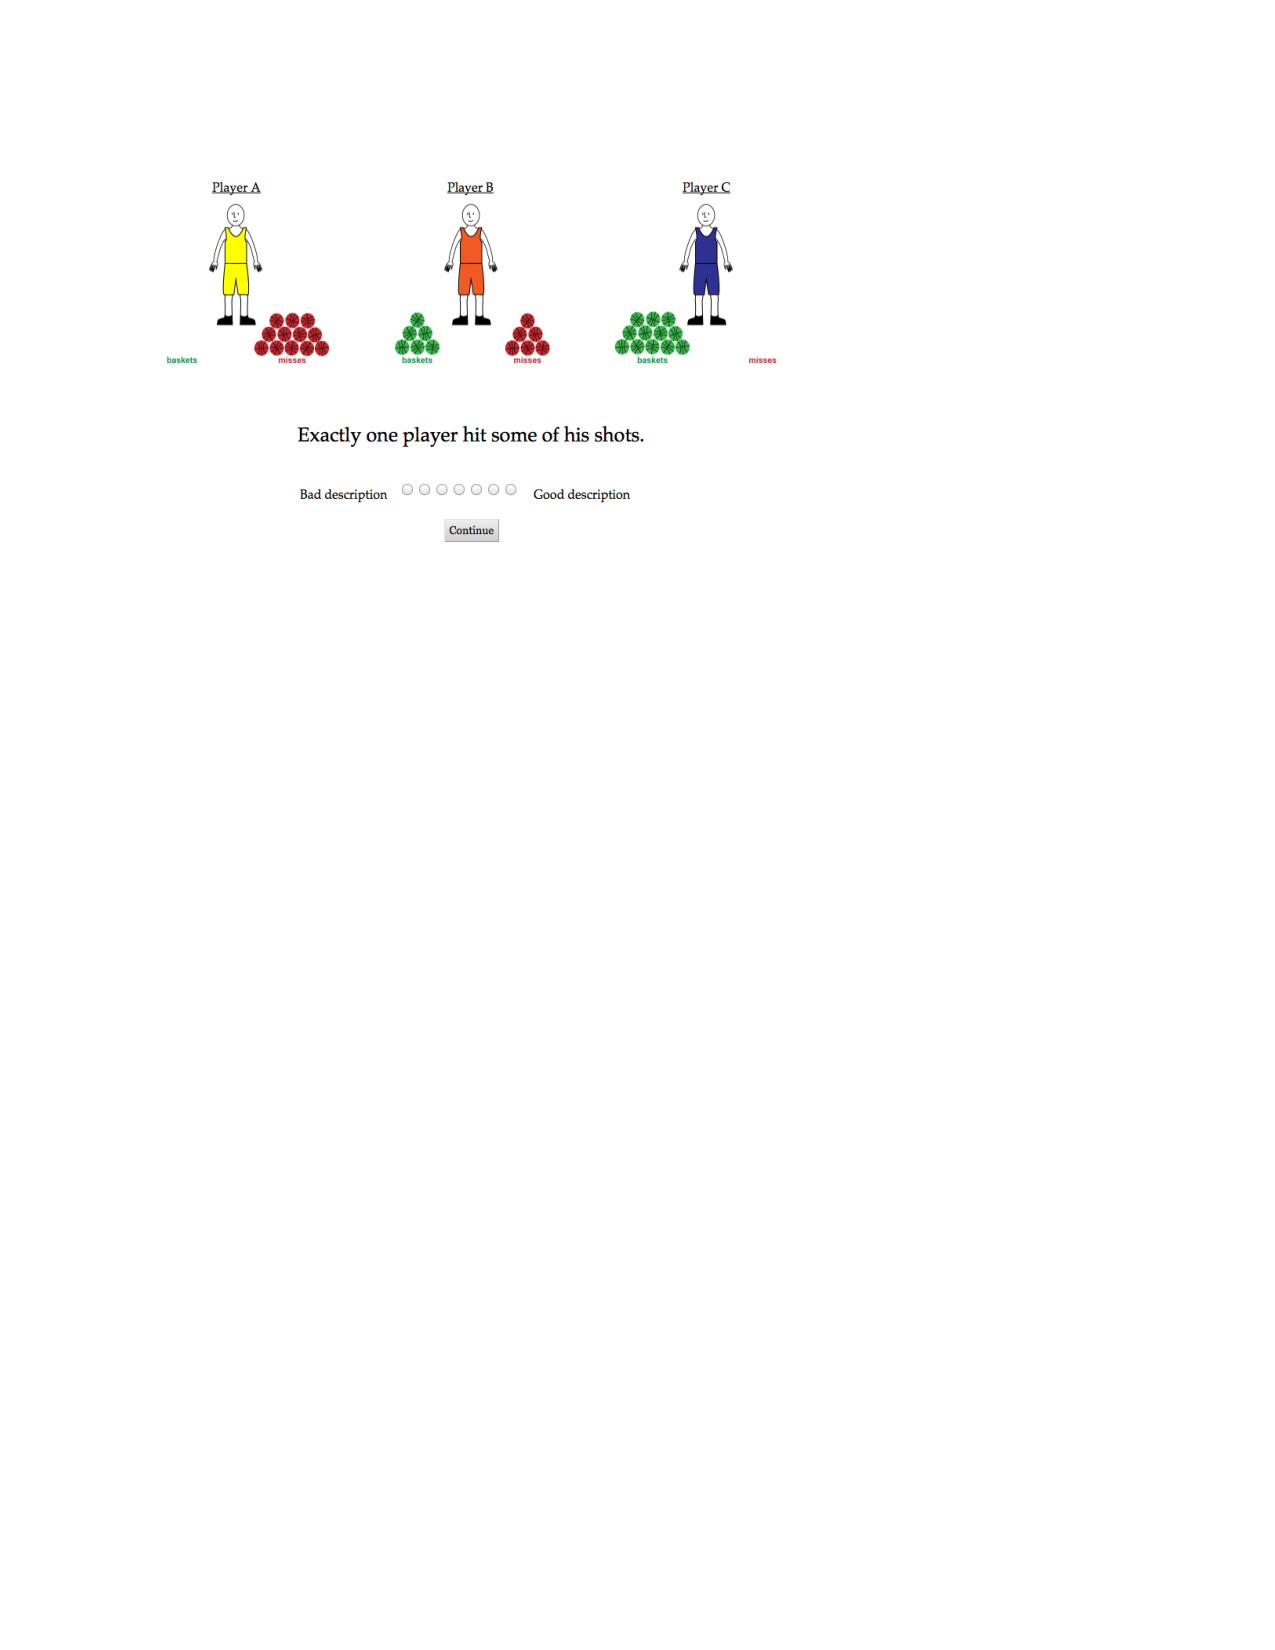
\includegraphics[width=0.85\textwidth]{fig/experiment-display}}
  \caption{Experiment 1 display.}
  \label{fig:exp1}
\end{figure}

The experiment had 300 participants, all recruited with Amazon's
Mechanical Turk. No participants or responses were excluded.  There
were 32 sentences, divided into 9 target sentences and 23 fillers. For
the target items, there were nine different conditions, corresponding
the worlds in \eg{conds}, in the notation we've been using to identify
possible worlds. 
%
\begin{examples}
\item\label{conds} $\set{\world{NNN}, \world{NNS}, \world{NNA},
    \world{NSS}, \world{NSA}, \world{NAA}, \world{SSS}, \world{SSA},
    \world{SAA}, \world{AAA}}$
\end{examples}
%
This is a subset of the full cross-product of the three outcomes
\world{N}, \world{S}, and \world{A} in which player $i$ always did at
least as well as player $i+1$, going left to right.  Our target
sentences are all quantified, so we don't care about the outcome for
any single player, meaning that we don't distinguish, e.g.,
\world{NNS} from \world{NSN}, allowing us to work with this smaller
set of conditions. In the experiment, the `order' of each world was
randomized, so that, e.g., the world type \world{NSA} appear visually
in all three of its orders.  The design was between-subjects: no
experimental participant judged the same sentence twice. Each sentence
received a total of 300 responses. For the target sentences, each
sentence--condition pair received between 19 and 44 responses (mean
30); this minor variation is the result of idiosyncrasies in the way
participants were assigned to the experiment. All the materials and
response data are available at the website for this paper.

As noted above, the design owes a debt to the previous work of
\citet{Geurts:Pouscoulous:2009} and \citet{Chemla:Spector:2011}, and
there is an obvious correspondence between their stimuli, which
involve geometric shapes, and our tournament displays. Our intuition
is that our displays place fewer cognitive demands on participants,
allowing them to concentrate on how well the sentences identify the
world. In addition, our displays introduce fewer points of variation
that are irrelevant for the experiment. For example,
\citet{Chemla:Spector:2011} use wheel-like displays in which, in the
crucial item, a single spoke extends from the vertex to a point on the
diameter. There are potentially many ways this state can be
drawn. With our displays, it was straightforward to show participants
every relevant variant of the condition, which allowed us to
factor out this kind of variation in our analyses. Our
expectation was that these changes to the original design would yield
a clearer overall picture.

%=====================================================================

\subsection{Results}\label{sec:exp1:results}

\Figref{fig:exp1-results} summarizes the responses by target sentence
and condition. The overall pattern shows that participants accurately
perceived whether the sentence was true or false; sentences that are
false on their literal interpretation always received average ratings
around 1 (the lowest point on the scale), and sentences that are true
on their literal interpretations were correspondingly given very high
ratings.

The responses strongly suggest that subjects reliably enriched the
scalar term in the scope of the monotone quantifier \word{every
  player} (top right panel). This sentence, which we discussed in
\secref{sec:implicature}, received its highest ratings in the
\world{SSS} condition, where local enrichment is needed in order for
the sentence to count as a complete report. Its ratings were also high
in the conditions mixing \world{S} and \world{A}, and its ratings were
extremely low for all other worlds. In other words, subjects gave low
ratings where the sentence was false, high ratings where it was true,
and especially high ratings where it could be construed with a local
implicature.

The pattern for \word{Exactly one player made some of his shots} is
more complex. As we discussed in \secref{sec:implicature},
\citeauthor{Chemla:Spector:2011} show that this kind of example makes
the most compelling case for local enrichment. This sentence received
its highest ratings in the the \world{NNS} condition/world, where it
is true under its literal and local enrichment construals. However, it
also received high ratings in the \world{NSA} and \world{SAA} worlds,
where it is true only with local enrichment. This is because two players made at
least some of their baskets in these worlds, ruling out the literal construal.  We
note also that its more strictly truth-conditional interpretation
seems to be salient as well, as it was rated highly on average in the
\world{NNA} condition.

\begin{figure}[tp]
  \centering
  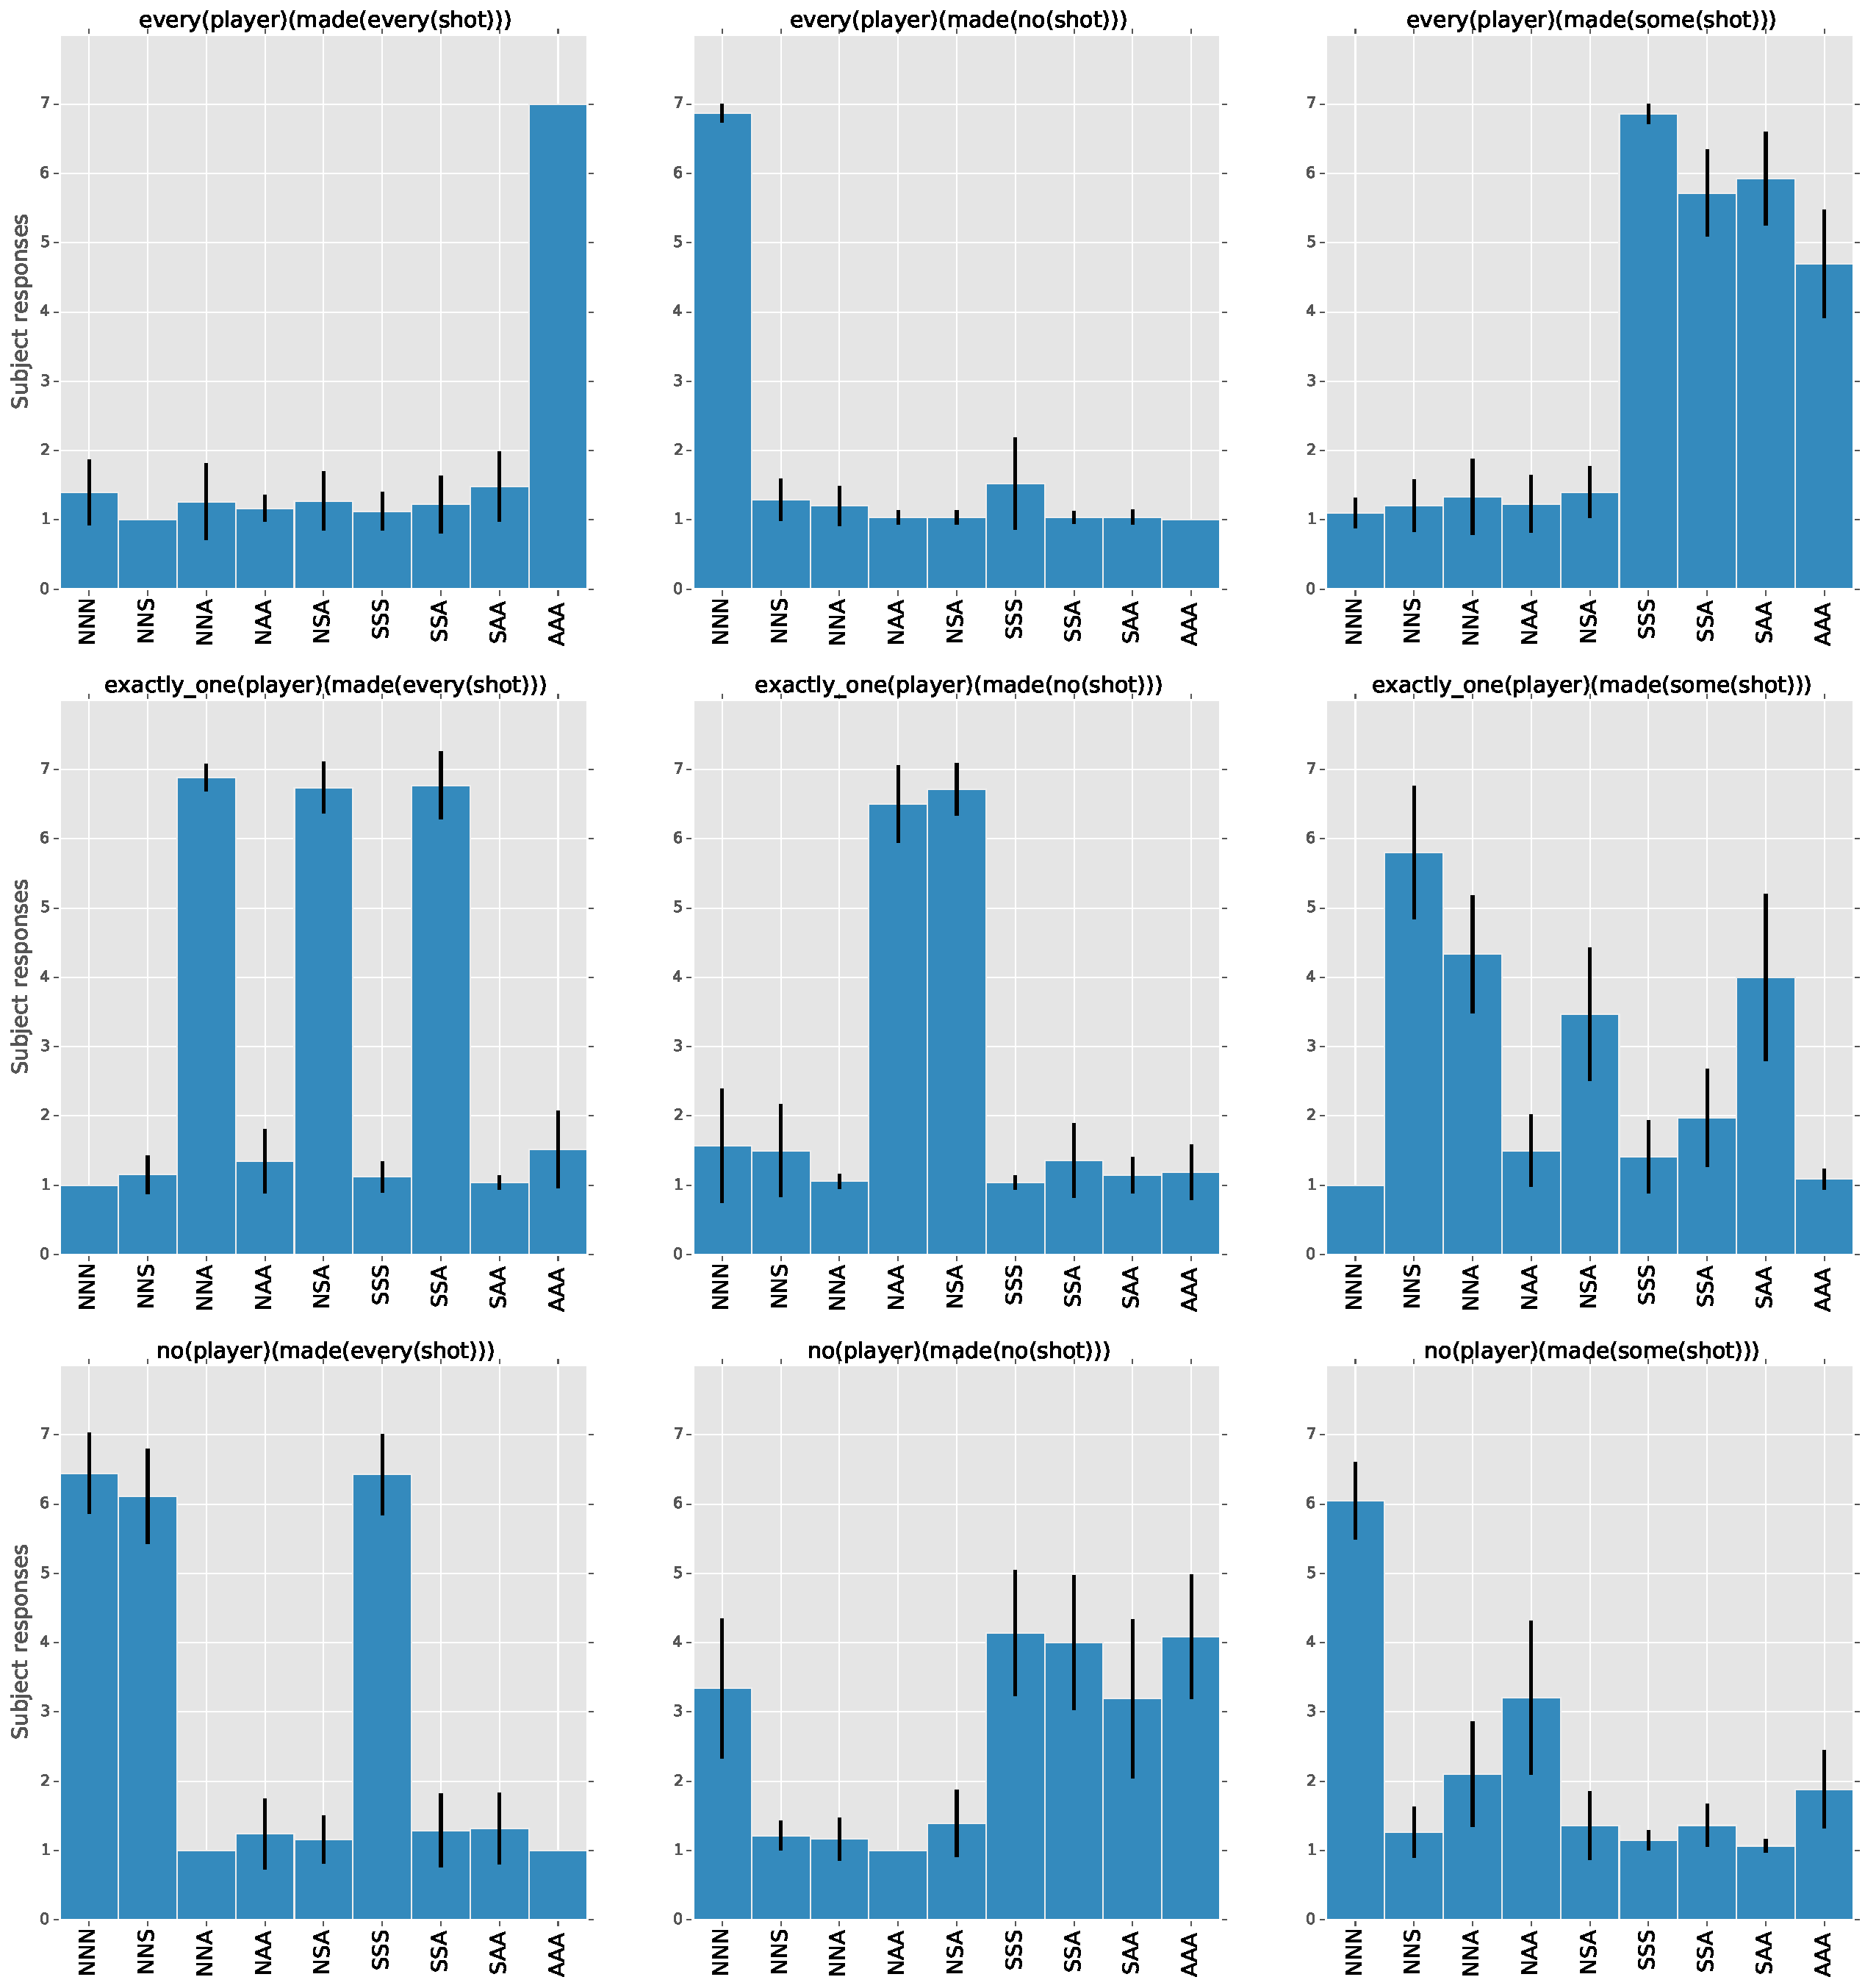
\includegraphics[width=1\textwidth]{fig/basketball-pilot-2-11-14-results-parsed}
  \caption{Experiment 1 results by target sentence.}
  \label{fig:exp1-results}
\end{figure}

\begin{figure}[t]
  \centering
  \begin{subfigure}{0.47\textwidth}  
    \centering
    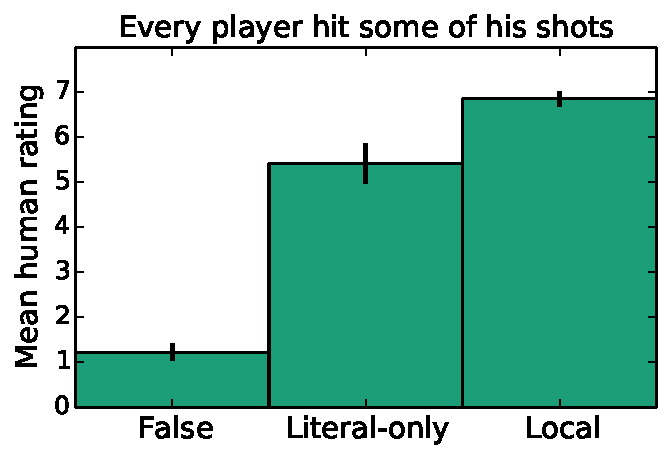
\includegraphics[height=2.8cm]{fig/every-some}
    \caption{False: any world containing \world{N}; 
      Literal-only: any true world containing \world{A}; 
      Local: $\set{\world{SSS}}$.}
    \label{fig:crucial-every}
  \end{subfigure}
  \hfill
  \begin{subfigure}{0.47\textwidth}
    \centering
    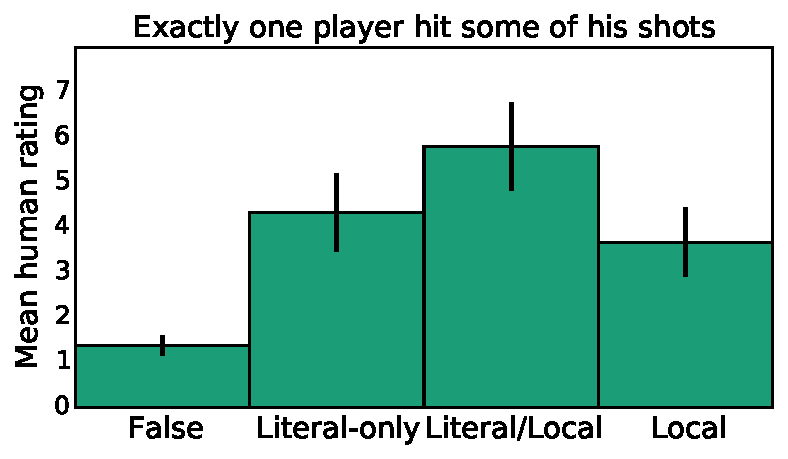
\includegraphics[height=2.8cm]{fig/exactlyone-some}    
    \caption{False: $\set{\world{NNN}, \world{NSS}, \world{SSS}, \world{SSA}, \world{AAA}}$;
      Literal-only: $\set{\world{NNA}}$;
      Literal/Local: $\set{\world{NNS}}$;
      Local: $\set{\world{NSA}, \world{SAA}}$.}
    \label{fig:crucial-exactlyone}
    \end{subfigure}
    \caption{Patterns for the crucial embedded scalar cases.}
    \label{fig:crucial}
\end{figure}

\marginpar{Might be reassuring to do some stats hypothesis testing related to \figref{fig:crucial}.}

For these two crucial items, we would like to get a clearer picture of
how the ratings compare across world-types that distinguish among the
different readings. \Figref{fig:crucial-every} and
\figref{fig:crucial-exactlyone} display the results of clustering the
worlds in ways that are informative for each sentence. In
\figref{fig:crucial-every}, the preference for local enrichment seems
clear; the only complication is that the single `Local' world,
\world{SSS}, is also one that makes the literal reading
true. Nonetheless, we venture that the high ratings are related to the
fact that there is a construal of the sentence that describes the
world as well as these quantified statements can. As we noted in
\secref{sec:implicature}, this case does not distinguish purely
Gricean accounts from grammar-driven ones, but it is noteworthy
nonetheless: our sportcaster scenario was designed to encourage
implicatures (the sportscaster should give informative reports), and it
seems to have done that.

For the case of \word{exactly one} over \word{some}, the pattern is
more complicated. Literal-only and local-only readings seem about
equally salient. The highest ratings come where both readings are
true, which echoes \posscitet{Chemla:Spector:2011} auxiliary
hypothesis that high ratings will correlate with high numbers of true
readings. However, the wide margin between `False' worlds and `Local'
worlds is very strong evidence that local readings are available ---
without the local construal, the sentence would be false in these
worlds. 

We conclude from these response patterns that local enrichment is
possible even in non-monotone environments, vindicating the guiding
hypotheses of \citet{Chemla:Spector:2011}. However, our primary
concern is not whether such readings are possible or impossible in a
binary sense, but rather how accurately we can predict them on the basis of contextual and world knowledge. In this
way, our objectives are more closely aligned with Griceans like
\citet{Geurts09}, \citet{Geurts:Pouscoulous:2009}, and
\citet{geurts-vantiel:2013:scalar}. We turn now to the task of
assessing the ability of our model from \secref{sec:model} to predict
both the quantitative and qualitative patterns in this experimental
data.

%=====================================================================

\subsection{Pragmatic model assessment}

To assess our pragmatic model, we simply run the uncertainty
model in the following setting, using messages derived from the
interpreted grammar in \figref{fig:grammar}.

\begin{examples}
\item\label{expmod}
  \begin{examples}
  \item $\Domain = \set{\playera, \playerb, \playerc}$
  \item $\Worlds = $ the set in \eg{conds}
  \item $\Refinable = \set{\word{some}}$
  \item $\Messages =
    \setlength{\arraycolsep}{2pt}
    \set{
      Q(\word{player})(\word{made}(S(\word{shot}))) :
      \begin{array}{l}        
        Q \in \set{\word{exactly one}, \word{every}, \word{no}}, \\
        S \in \set{\word{every}, \word{no}, \word{some}}
      \end{array}}$
  \item $\Costs(\nullmsg) = 5$; $\Costs(\msg) = 0$ for all $\msg \in \Messages-\set{\nullmsg}$  
  \item $\StatePrior(w) = \StatePrior(w')$ for all $w, w' \in \Worlds$
  \item $\LexPrior(\Lex) = \LexPrior(\Lex')$ for all $\Lex, \Lex' \in \LexSet$
  \end{examples}
\end{examples}

\marginpar{\Figref{fig:exp1-corr} is not especially informative or helpful about our analysis. This could be due to a simplistic linking hypotheses. Sorting this out is an urgent to-do.}

\begin{figure}[t]
  \centering
  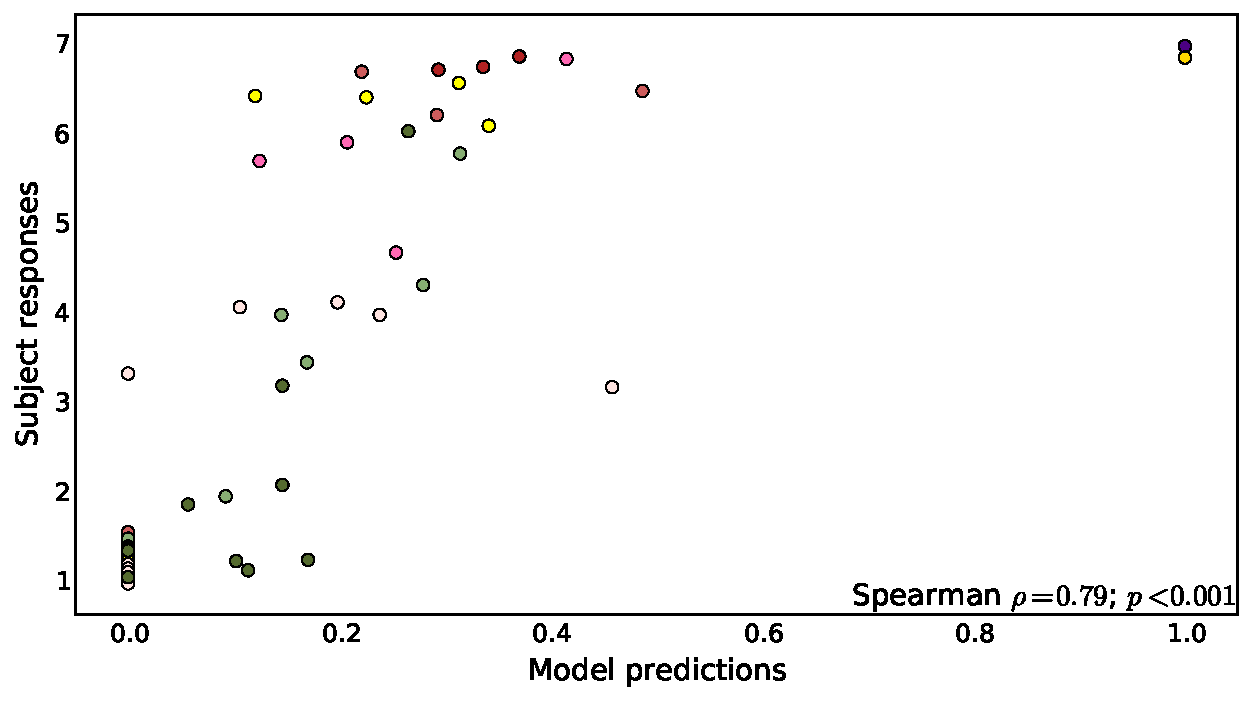
\includegraphics[width=0.7\textwidth]{fig/experiment-scatterplot}
  \caption{Experiment 1 analysis: correlating model predictions
    (x-axis) with human responses (y-axis) for each
    sentence--condition pair.}
  \label{fig:exp1-corr}
\end{figure}

The predictions of the model are summarized with the correlation
analysis in \figref{fig:exp1-corr}. The model predictions are
given on the $x$-axis and the mean human responses are given
on the $y$-axis. The overall correlation is $0.8$ ($p < 0.001$).

\begin{figure}[t]
  \centering
  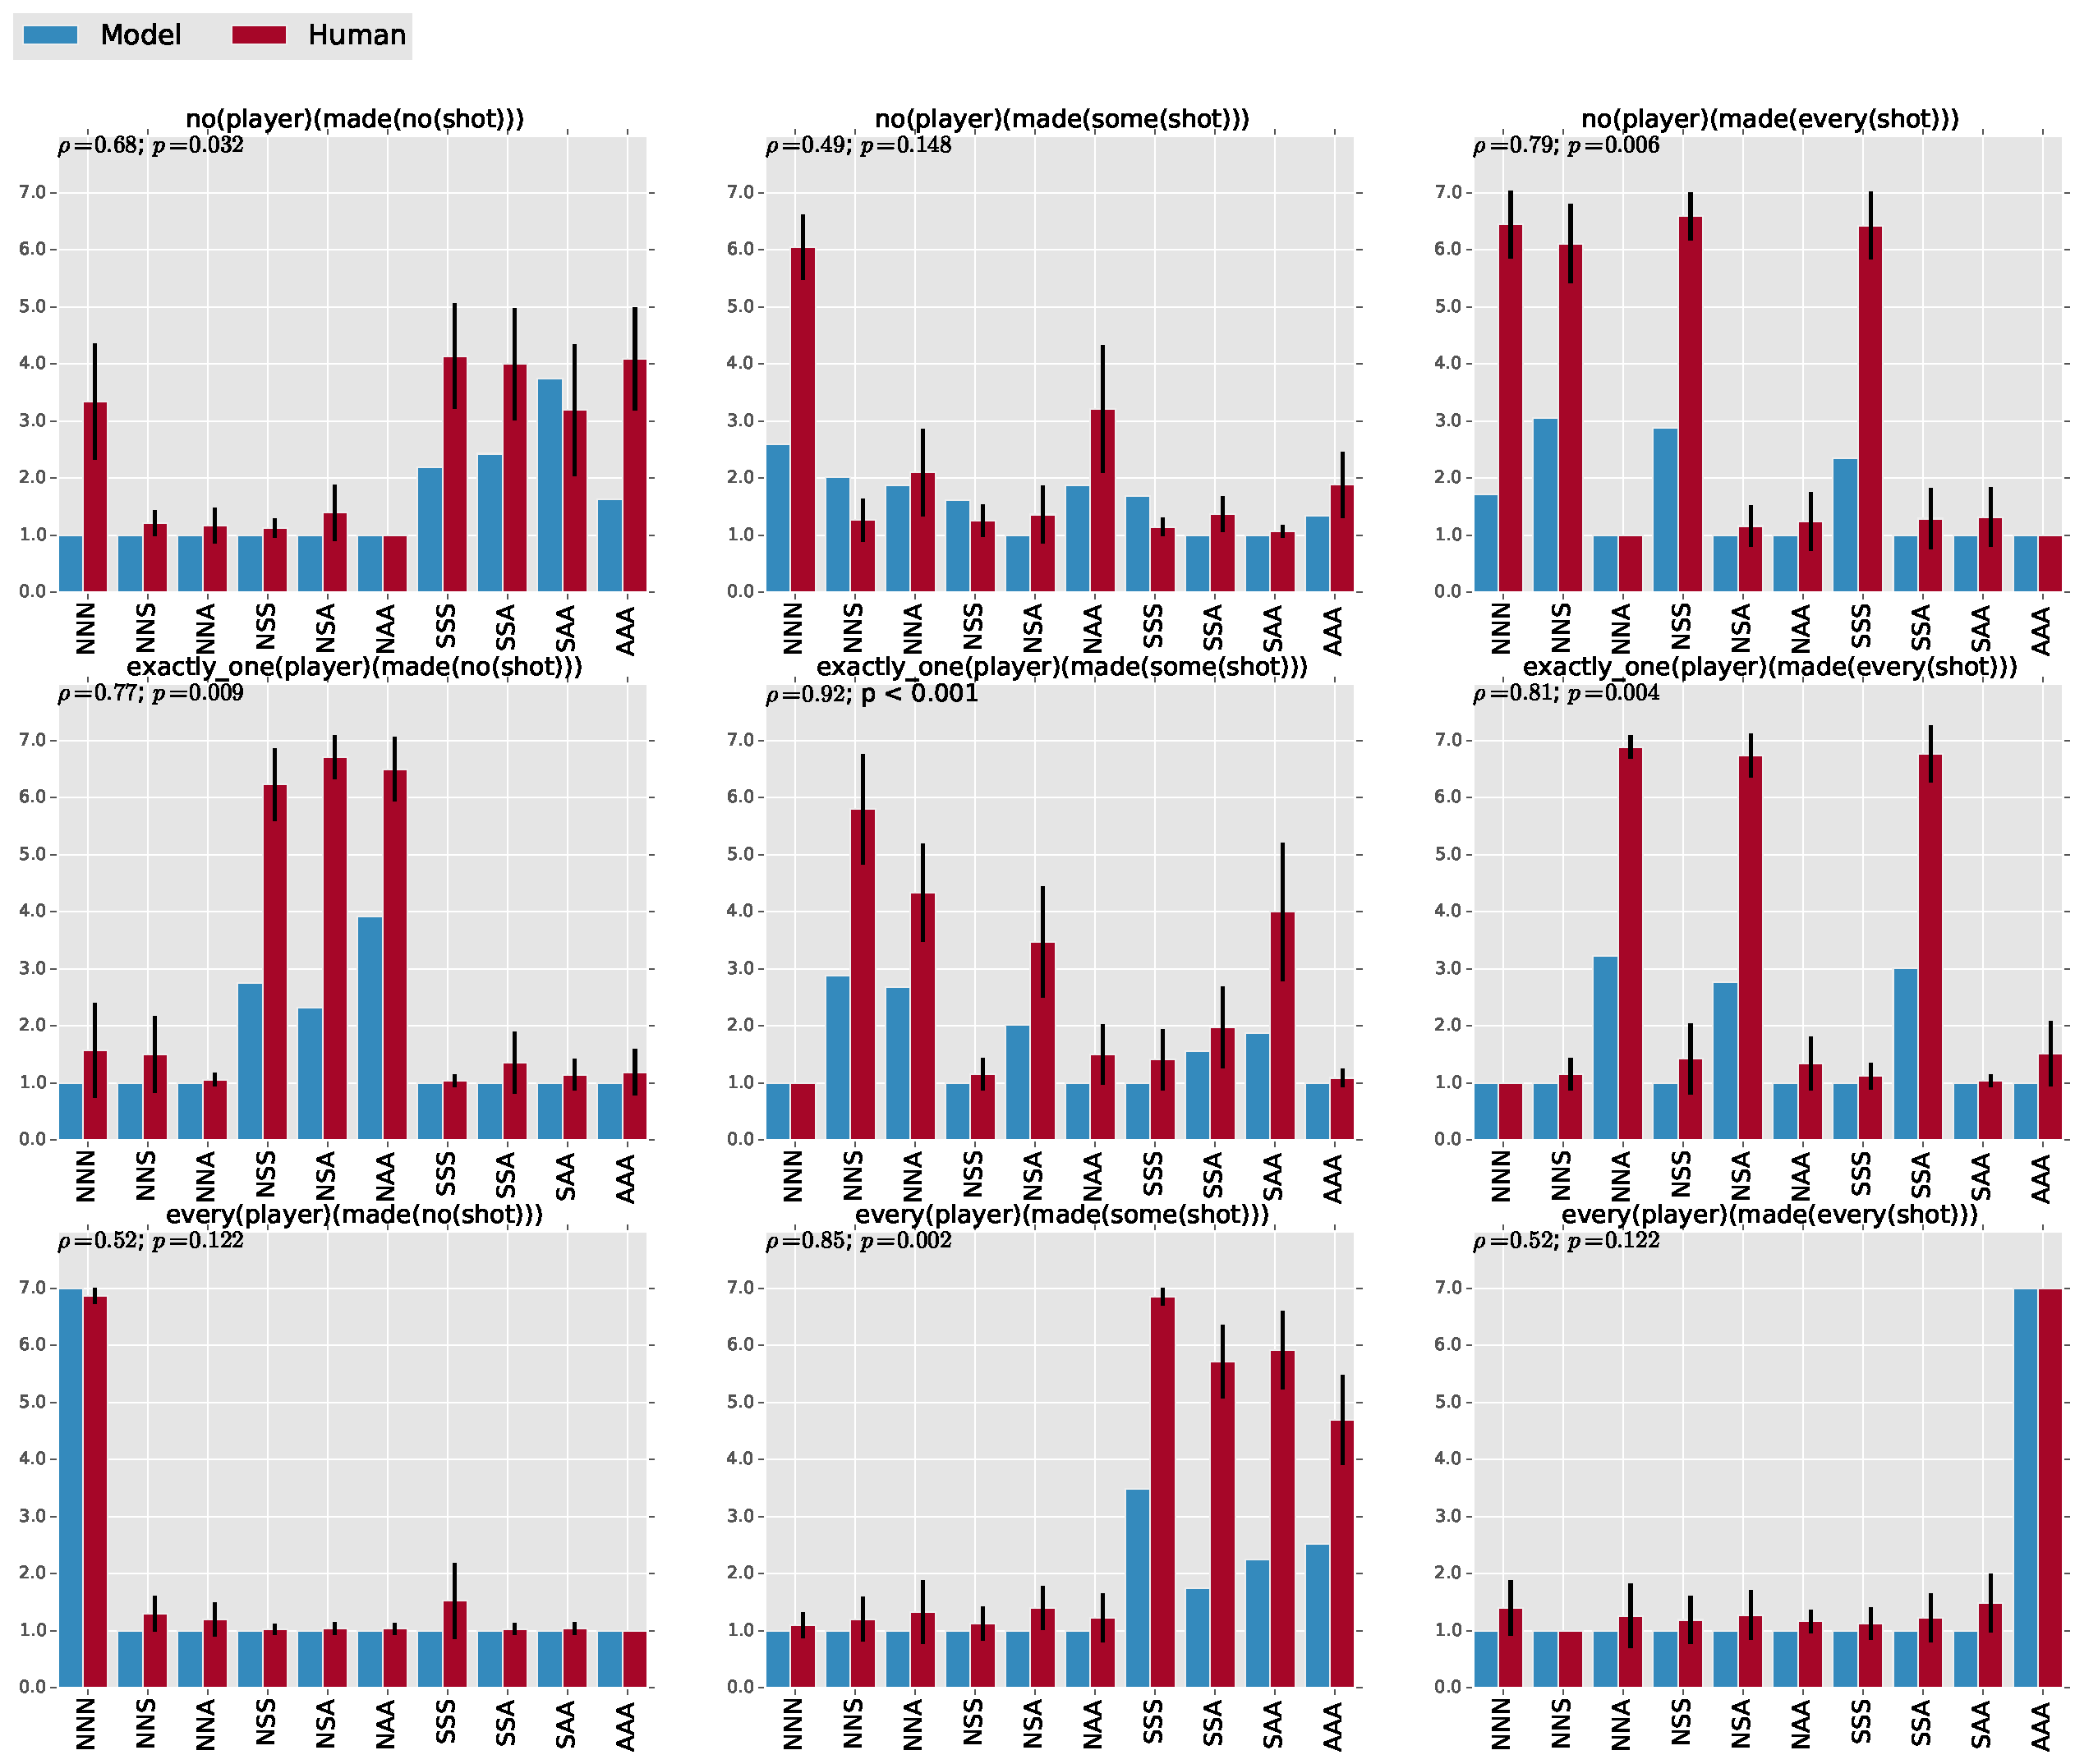
\includegraphics[width=1\textwidth]{fig/experiment-barplots}
  \caption{Experiment 1 analysis by target sentence, comparing model
    predictions (green) with human responses (orange).  The model
    predictions are transformed into the Likert space using the
    rescaling in \eg{likert}. They remain lower than the human
    responses because they are constrained to form a probability
    distribution, whereas the human responses are not.}
  \label{fig:exp1-analysis}
\end{figure}

The predictions for each of the nine messages are given in
\figref{fig:exp1-analysis}, alongside the summary of human responses
from \figref{fig:exp1-results}. Each panel includes the Spearman
correlation coefficient and associated $p$-value. The model
predictions have been mapped into the Likert space of the human
responses by the linear transformation \eg{likert}; this does not
affect the statistical testing we report; it simply makes it easier to
compare the values side-by-side (though the model values still remain
lower because they are normalized into a probability distribution,
whereas the human responses are not so constrained).
%
\begin{examples}
\item\label{likert} $\Likert(p) = 1 + 6p$
\end{examples}

\marginpar{These analyses worry me because of the bimodal distribution of the 
predictions and response data. It raises concerns about Type~I errors.}

Overall, the correlations are extremely high. Only the negative
sentences have comparably low values, possibly because of ambiguities
that we did not seek to model. The sentence containing two negatives
resulted in a somewhat chaotic-looking distribution of
middle-of-the-scale judgments in true worlds.\marginpar{I don't think it's so chaotic - the main issue other than scope/PPI is that some people gave a negative concord intepretation to no/no, so that NNN got decent ratings.} And the example with
\word{no} in subject position and \word{some} in object position may
have a scope ambiguity that we did not model. In particular,
\word{some} is often classified as a positive polarity item, resistant
to staying in the semantic scope of negative morphemes
\citep{Baker70,Israel96}, whereas our model simply gives it narrow
scope.  These two cases are responsible for bringing down the overall
correlation in \figref{fig:exp1-corr}.

\begin{figure}[t]
  \centering
  \begin{subfigure}{0.48\textwidth}
    \centering  
    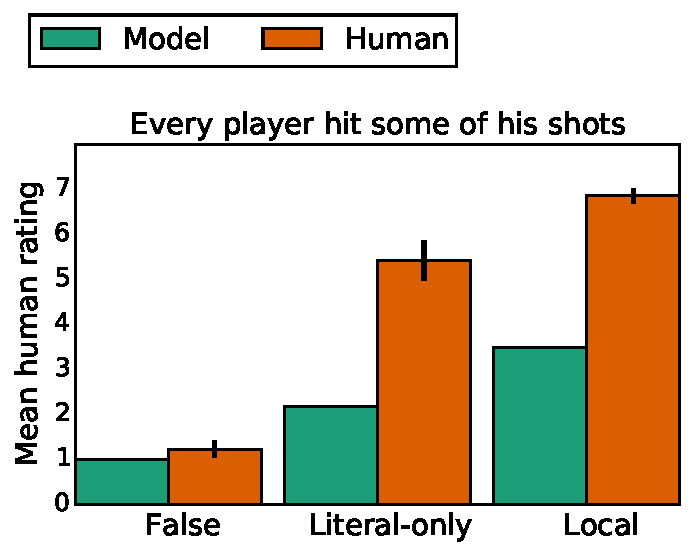
\includegraphics[height=4cm]{fig/every-some-modcmp.pdf}
    \caption{\word{every}/\word{some}.}
    \label{fig:modcmp-everysome}
  \end{subfigure}
  \hfill
  \begin{subfigure}{0.48\textwidth}
    \centering  
    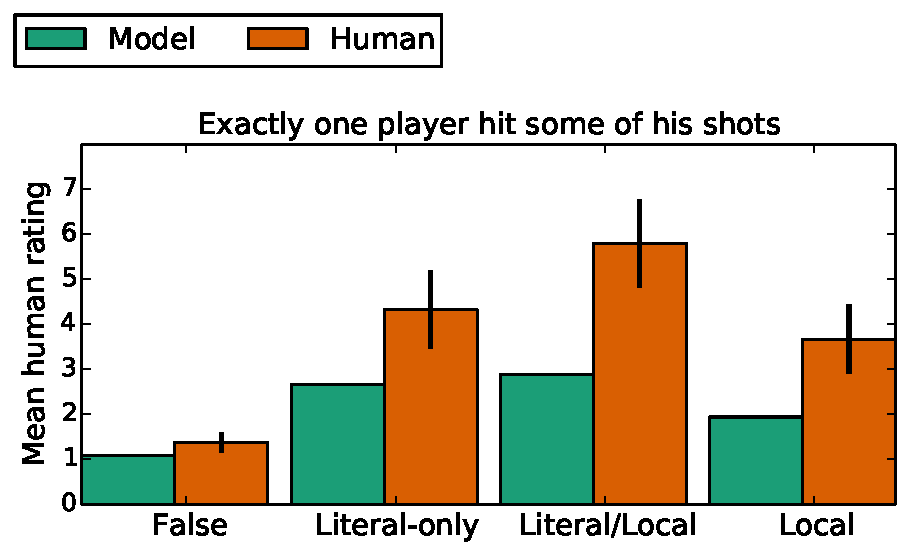
\includegraphics[height=4cm]{fig/exactlyone-some-modcmp.pdf}
    \caption{\word{exactly one}/\word{some}.}
    \label{fig:modcmp-exactlyonesome}
  \end{subfigure}
  \caption{Comparing model and human data for the two embedded scalar cases.}
  \label{fig:modcmp-crucial}
\end{figure}


Importantly, for our two crucial test cases (top right and middle
right), the model predictions are extremely well-correlated with the
human pattern. The picture is summarized in
\figref{fig:modcmp-crucial} using the same grouping of
worlds/conditions from \figref{fig:crucial}. For both items, our model
predicts the same ranking of conditions by preference; the Pearson
rank correlation coefficient is $1$ in both cases. In this sense, the
model not only captures the qualitative pattern of preferences, but
also achieves a good fit with the quantitative pattern we observe in
the human data.

\marginpar{It's too bad that we don't have experiments on the influences of competitors like this. It seems more relevant to our model than the focus/only stuff. Could be hard to design, though.}

Our model's performance is sensitive to the space of competitor
messages, so it is worth asking how robust these findings are to
changes in this area. We have found that the basic pattern is robust
to a number of changes to the space of quantifiers, and we invite
readers to further explore the space using our implementation.  The
only noteworthy finding we have to report in this regard is that
allowing \word{exactly one} into object position has a major impact:
while \world{SSS} remains the best-guess inference for the message
\word{every}/\word{some} in this setting, \word{exactly
  one}/\word{some} effectively loses its embedded implicature reading.
This makes intuitive sense given the nature of the model: if the
speaker has the option to choose \word{exactly one of his shots}, and
that form is equally costly, then surely her avoidance of that form in
favor of \word{some of his shots} is a signal that she regards the
local enrichment as infelicitous.


%%%%%%%%%%%%%%%%%%%%%%%%%%%%%%%%%%%%%%%%%%%%%%%%%%%%%%%%%%%%%%%%%%%%%%

\section{Experiment 2: focus and \word{only}}\label{sec:exp2}

\marginpar{I am not convinced that this experiment needs to be included. Its role is not especially clear.}

Experiment~2 used the same design, materials, and display as
experiment 1, differing only in the following respect: the embedded
scalar term \word{some} was changed to `only some' in the `only'
condition and `\textbf{SOME}' in the `focus' condition. Our rationale
for running the experiment was twofold. First, including \word{only}
essentially turns the local implicature into an entailment; there is
some indeterminacy introduced by the context-dependence of the
discourse particle \word{only}, but our contexts essentially force a
construal as \word{only some} ranging over shots.  Second, even though
\CFS\ are cautious about linking their $O$ operator to \word{only},
the formal parallels seem genuine. This leads us to expect that focus
might be a good, albeit indirect, method of signaling that a local
implicature is intended. We therefore expect focus to increase the
rates of such readings.

\marginpar{Numbers need to be checked. Is the variation in response counts really this high? 14-44 seems like a large range.}

We had 600 Mechanical Turk workers take part in the experiment; we
solicited 312 responses per sentence, where the `focus' and `only'
version of the \word{some} sentence are each different sentences.
Each sentence--condition pair received 14--44 responses. The results
are we would expect: prosodic focus did in fact boost the signal of
the embedded implicatures somewhat, and including \word{only}
increases it still more. \Figref{fig:expcmp} shows the two crucial
items alongside the original data from \figref{fig:crucial}. For
\word{every} in subject position, the rate of local implicatures was
already high, so there wasn't much room to move things around. For the
\word{exactly one} subject, though, the trends seem to be meaningful.

Our model once again achieves high correlations in the \word{only}
cases (correlation $0.77$; $p < 0.001$). We have not tried to model
the prosodic focus cases, because we do not have a clear idea about
how to represent it in our model. Our data and code are available for
further experimentation in this area.

\begin{figure}[t]
  \begin{subfigure}{0.48\textwidth}
    \centering  
    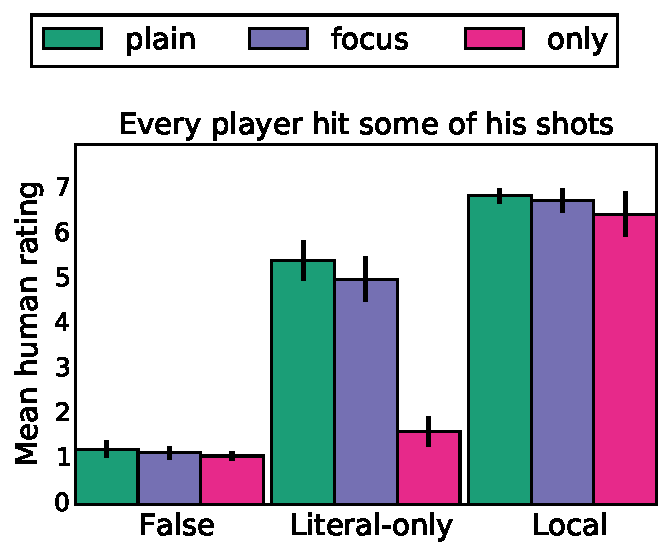
\includegraphics[height=4cm]{fig/every-some-expcmp}
    \caption{\word{every}/\word{some}.}
    \label{fig:expcmp-everysome}
  \end{subfigure}
  \hfill
  \begin{subfigure}{0.48\textwidth}
    \centering  
    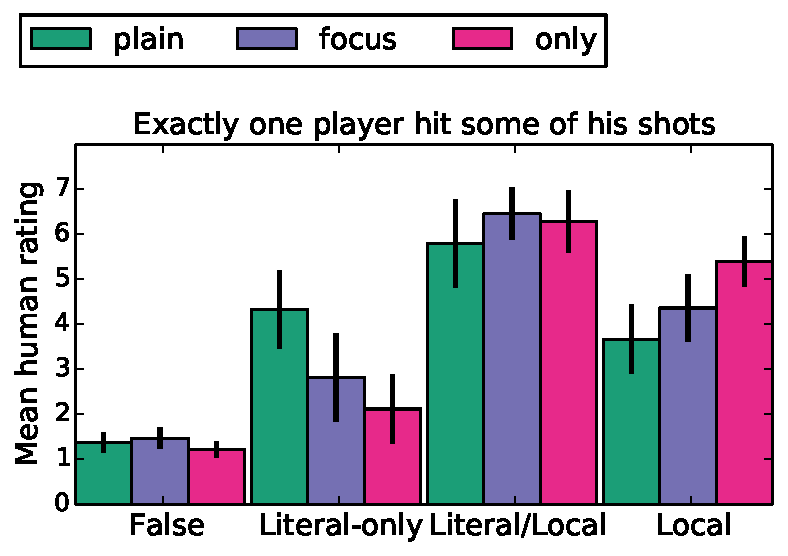
\includegraphics[height=4cm]{fig/exactlyone-some-expcmp}
    \caption{\word{exactly one}/\word{some}.}
    \label{fig:expcmp-exactlyonesome}
  \end{subfigure}
  \caption{Experiment comparisons of the effects of focus and
  \word{only} in the embedded scalar terms.}
  \label{fig:expcmp}
\end{figure}


%%%%%%%%%%%%%%%%%%%%%%%%%%%%%%%%%%%%%%%%%%%%%%%%%%%%%%%%%%%%%%%%%%%%%%

\section{Conclusion}\label{sec:conclusion}

With this paper, we sought a synthesis between Gricean, interactional
accounts of pragmatic reasoning and grammar-driven ones like that of
\citet{ChierchiaFoxSpector08}. It seems to us inevitable that both
grammar and interaction will play leading roles in the final theory of
these phenomena; at some level, all participants in the debate
acknowledge this. Our achievement is to bring what we regard as the
crucial components of these approaches together into a unified formal
model that makes quantitative predictions. The key components of the
model are lexical uncertainty and recursive modeling of speaker and
listener agents. The lexical uncertainty property is in evidence in
\citeauthor{ChierchiaFoxSpector08}'s account as well: underspecified
logical forms with context dependent meanings mean that each
expression potentially needs to have its meaning refined in context;
our model has similar formal mechanisms but offers an account of how
discourse participants to select among them.  The recursive reasoning
is characteristic of both Gricean approaches and signaling systems
approaches like that of \citet{Lewis69}; our model shares formal
properties of these approaches but makes quantitative predictions of
the sort that can be correlated with human preferences in
communication. There are by now many models in the same family as ours
(see, e.g., 
%
\marginpar{Add your favorite references here!}
%
\citealt{CamererHo:2004,Jaeger:2011,Smith:Goodman:Frank:2013,Kao-etal:2014}),
so further exploration is likely to yield an even more nuanced
picture. We have made publicly available all the data and code
associated with this paper, in an effort to encourage the development
of more theories of pragmatic reasoning as both semantic and
pragmatic.

%%%%%%%%%%%%%%%%%%%%%%%%%%%%%%%%%%%%%%%%%%%%%%%%%%%%%%%%%%%%%%%%%%%%%%

\bibliographystyle{apalike}
\bibliography{embedded-scalars-bib}

\end{document}

